
\documentclass[12pt,bibliography=totoc]{article}

\usepackage{graphicx}
\usepackage{times}
\usepackage{changepage}
\usepackage{textgreek}
\usepackage{amsmath}
\usepackage[left=2.5cm, right=2.5cm, top=2.5cm, bottom=2.5cm]{geometry}
\usepackage{amsmath}
\usepackage{booktabs}
\usepackage{array}
\usepackage{float}
\usepackage{natbib}
\usepackage{fancyhdr}
\graphicspath{ {./images/} }
\usepackage{placeins}
\usepackage{graphicx}
\usepackage{subcaption}
\usepackage{setspace}
\singlespacing
\usepackage{booktabs,amsfonts,dcolumn}
\newcolumntype{d}[1]{D..{#1}}
\newcommand\mc[1]{\multicolumn{1}{c}{#1}} % handy shortcut macro
\usepackage[justification=centering]{caption}
\usepackage[colorlinks=true,allcolors=blue]{hyperref}%
\usepackage{graphicx}
\usepackage{tabularx}
\usepackage{tikz}
\usepackage[toc, page]{appendix}
\usepackage[nottoc]{tocbibind}
\usepackage{indentfirst}
\usepackage{caption}
\usepackage{booktabs}
\usepackage[flushleft]{threeparttable}



\newcommand\fnote[1]{\captionsetup{font={it,small} }\caption*{#1}}

\pagestyle{fancy}
% Clear the header and footer
\fancyhead{}
\fancyfoot{}
% Set the right side of the footer to be the page number
\fancyfoot[R]{\thepage}



\begin{document}


\begin{titlepage}
  % \vspace*{\stretch{1.0}}
  % \begin{center}
   %   \Large\textbf{Országok és vállalatok multi-dimenziós összekötöttségének vizsgálata, különböző pénzügyi instrumentumok mentén}\\
    %   \bigskip
    %  \large\textit{Kotró Balázs}\\
    %  \medskip
    %  \large{Komplex vizsga - Kutatási tanulmány}
   %\end{center}
  % \vspace*{\stretch{2.0}}
%\end{titlepage}




 \begin{center}
\Huge\textbf{Interconnectedness Among Sovereign Yield Curve Factors - Working title}\\
 
\vspace{3cm}


 \Large\textit{Milan Csaba Badics - Balazs Kotro}
 
 \vspace{3cm}
 
\Large\textit{MKE Konferencia - draft version}


\vspace{4cm}
\end{center}

\begin{abstract}
We are investigating the interconnectedness of the yield curve factors of 12 developed economies worldwide. From the yield curve time series we extract the Level, Slope and Curvature factors by the Diebold-Li decomposition technique for every day. On the recieved 36 observation series a pairwise Toda-Yamamoto causality test is performed in order to identify connections. Our static results show that there is a significant amount cross connections among the different factos. On average Level is the most connected factor, followed by Slope and Curvature. We also identify the USA to be the main driver of the observation universe. Our dynamic results show that during turbulent economic periods the density of the connections gets higher. On the chosen time horizone, USD Level, USD Curvature and Norwegian Slope are the most interconnected factors.
\end{abstract}


\end{titlepage}

\newpage

\section{Introduction and literature review}

The subprime crisis renewed the interest in analyzing the co-movements of different financial instruments and systemic risk related studies came to the forefront. Shocks can be transmitted differently across various assets, therefore it is convenient to achieve awareness both for regulators and other market participanst in order to react more efficiently. Understanding such network structures are valuable for reducing potential damage and making appropriate future decisions. Analysis of the interconnectedness of different assets plays crucial role in systematic risk assessment. Furthermore, during crisises the strength of connections sharply increases and risk spills over across financial institutes and sovereign bonds, as it happened during the Financial Crisis of 2008-2009 and during the European Sovereign Crisis (\cite{diebold2012better}). %\textcolor{red}{IDE KELL MAJD HIVATKOZÁST KERESNI}

Since the financial system is a huge, complicated, interactive system, in recent years scholars began using complex network theories to investigate the interconnectedness of financial institutions. \cite{acemoglu2015systemic} points out that in smaller financial systems, shocks make the densely interconnected network steadier, however after a certain size the opposite applies. According to \cite{elliott2014financial}, diversification initially allows failure cascades to travel within the system, but as it increases further, organizations are better insured against anothers' failures. Depending more on other participants makes personal sensitivity lower on own investments. %\textcolor{red}{SZERINTEM ITT VAN MÉG 1-2 FONTOS CIKK RÁNÉZEK MAJD}

In the empirical literature there are several methods to measure connectedness. In the last decade the widespread methods are Granger causality network (\cite{billio2012econometric}), CoVaR (\cite{adrian2008federal}), MES (\cite{acharya2012capital}) and numerous studies appeared based on the Vector AutoRegressive Diebold-Yilmaz (DY) framework (\cite{diebold2009measuring}, \cite{diebold2012better}). Compared to CoVaR and MES methods, the advantage of Granger causality based frameworks is the ability to examine the network both on micro (pairwise connectedness) and macro (total connectedness) level. As result, these methods have been often used to analyse the network on different asset classes like equities, bonds, exchange rates or commodity prices. Most analysis focuses on the whole system or some subpart. The dynamics of individual assets' role in the system have not been explored yet. %\textcolor{red}{IDE KELL hivatkozások összeszednem}

%\smallskip{}
%\textcolor{red}{KELLENE EGY KOINTEGRÁCIÓT Nem szokta vizsgálni bekezdés}
%\smallskip{}

Central banks traditionally rely on the co-movements of different maturities of yield curves to make effective monetary policy decisions. According to the expectations hypothesis, long-term interest rates are influenced by current and expected future short-term interest rates. However, increasing globalization of financial systems and structural changes across economies have disrupted the integration of the maturity spectrum of different yield curves. Short-end movements are more exposed to monetary policy decisions, so their interconnectedness is more consistent with the alternation of business cycles. The long end of the yield curve is mainly affected by global investment, with current preferences and risk appetite being the primary drivers. The integration of distant maturity points is driven by global capital flows and the volume of investments. %\textcolor{red}{IDE MINDENKÉPP KELLENEK HIVATKOZÁSOK}

Usually, a tenor structure consists of multiple maturities which means one-one individual time series. It is challenging to deal with such a magnitude of data, therefore in raw format the yield curve itself is not used. \cite{fernandez2016using} examines only the 10Y yield curve point on EMU countries while \cite{claeys2014measuring} choose the spread between EU government bond yields and German sovereign bond yield, also considering 10 years of maturity. \cite{ahmad2018financial} pick bond indices to analyze and \cite{sowmya2016linkages}
decompose the yield curve to Level, Slope and Curvature factors with the Diebold-Li dimension reduction technique. 

We are eager to find the less and most interconnected participants of our system, via understanding the connections not only between particular factors, but involving all three of them. We are also curious for the behavior of such linkages during time, thus besides static analysis we performed rolling window-based tests as well. Our contribution to the existing literature is fourfold. We analyze the interconnectedness of different yield curve factors with the consideration of cointegration among the time series. This is the first study which examines the crosswise causality connections among Level, Slope and Curvature. We choose developed economies from all over the World in order to achieve a wide geographical coverage. %\textcolor{red}{ITT LEHET KELLENE MÉG MAGYARÁZAT}

We find that there is cointegration between the yield curve factors, therefore our modelling approach (Toda-Yamamoto method) is justified. There is a not negligible amount of significant cross connections among these factors. The Level drives the highest number of linkages while the Curvature is the main receiver. Slope is ranked as second in both comparisons. USD factors have the most net connections (outgoing – incoming) thus it can be considered as the main driver of the system. Our dynamic approach shows that during a recession period the sum of the connections in the network increases which statement is supported with different window sized robustness checks.


%\section{Literature review}

%There are a few pioneer studies about the intedependence of the sovereign bond market.
%\cite{ilmanen1995time} examines the predictable variation in long-maturity government bond returns in six countries using a linear regression model with local and global instruments. 
%\cite{clare2000analysis} decompose the relationship between the government bond markets of Germany, the United Kingdom, and the United States. They find that global factors influence the yield curves for each of these markets and the impact of these factors increases significantly during times of financial stress.
%\cite{driessen2003common} estimate and interpret the factors that jointly determine bond returns of different maturities in the US, Germany, and Japan. They find that the positive correlation between bond markets is driven by the term structure levels, not by term structure slopes. 
%\cite{dewachter2004effect} develop a benchmark against which the effects of ECB (European Central Bank) monetary policy on the German bond market can be evaluated. They find that yield spreads increased substantially during the EMU (European Monetary Union) period. 
%\cite{laopodis2004monetary} examines the monetary policy implications of the greater integration of the capital markets using long-term interest rates. He finds greater convergence among countries in the EU (European Union)
%as Germany still retains its hegemonic status.

%There are papers on sovereign yield spreads. 
%\cite{balli2009spillover} examines the time-varying nature of European government bond market integration by employing multivariate GARCH models. He states that global factors are sufficient for the volatility of yield differentials among euro government bonds. 
%\cite{favero2012sovereign} provide new evidence on the determinants of sovereign yield spreads and market sentiment effects in the Eurozone to evaluate the rationale for a common Eurobond jointly guaranteed by Eurozone member states. 
%\cite{antonakakis2013sovereign}examine sovereign bond yield spread spillovers between Eurozone countries using the VAR-based spillover index model of \cite{diebold2012better} and impulse response analyses. Their findings highlight the increased vulnerability of the Eurozone from the destabilizing shocks 
%originating mostly from the Eurozone countries in the periphery and to a lesser extent from the Eurozone core. 
%\cite{costantini2014determinants} find that fiscal imbalances – namely expected government debt-to-GDP differentials – are the primary long-run drivers of sovereign spreads.

%The literature on volatility spillovers in bond markets is scanty. 
%\cite{skintzi2006volatility} examine dynamic linkages among the European bond markets. They find that significant volatility spillovers exist from both the aggregate Euro and US bond markets to the individual European markets. They also conclude that the introduction of the Euro has strengthened the volatility spillover effects and the cross-correlations for most European bond markets. 
%\cite{christiansen2007volatility} examines volatility spillover from the US and aggregate European bond markets into individual European bond markets using a GARCH volatility-spillover model. Results indicate that for EMU countries, the US volatility spillover effects are rather weak (in economic terms) whereas the European volatility spillover effects are substantial. The bond markets of EMU countries exhibit high integration after the introduction of the euro. The post-Euro period has further strengthened the integration process. They find interest rate convergence as one of the primary drivers of bond market integration.

%\cite{gomez2014update} apply the Granger-causality approach and endogenous breakpoint test to offer an operational definition of contagion to examine (EMU) countries public debt behaviour. A database of yields on 10-year government bonds issued by 11 EMU countries covering fourteen years of monetary union is used. The main results suggest that the 41 new causality patterns, which appeared for the first time in the crisis period, and the intensification of causality recorded in 70\% of the cases provide clear evidence of contagion in the aftermath of the current euro debt crisis. 
%\cite{sibbertsen2014testing} study tests for a break in the persistence of EMU government bond yield spreads examining data from France, Italy and Spain and using German interest rates as a kind of benchmark. Their results provide evidence for breaks between 2006 and 2008. The persistence of the yield spreads against German government bonds has increased significantly after this period.

%Besides this, few studies have also examined volatility spillovers in bond markets using \cite{diebold2009measuring}, \cite{diebold2012better} methodology. 
%\cite{claeys2014measuring} measure direction and extent of sovereign bond markets linkages among sixteen EU (European Union) using a factor-augmented version of the VAR model in \cite{diebold2009measuring}. 
%\cite{fernandez2015volatility} examine volatility spillovers in EMU sovereign bond markets. They find that slightly more than half of the total variance of the forecast errors is explained by shocks across countries rather than by idiosyncratic shocks. They also report that during the pre-crisis period, most of the triggers in the volatility spillovers were central EMU countries – peripheral countries imported credibility from them – while during the crisis, peripheral countries became the dominant transmitters. 
%\cite{fernandez2016using} examine the time-varying behavior of net pair-wise directional connectedness at different stages of the recent sovereign debt crisis.



\section{Methodology}
\noindent
\subsection{The Nelson-Siegel yield curve model and the Diebold-Li decomposition}


%A hozamgörbe modelleknek az a célja, hogy lehetővé tegyék a hozamgörbe illesztését, ezt követő paraméteres struktúrán alapuló interpolációját és extrapolációját, amely megegyezik más, nem parametrikus (statisztikai alapú) illesztési modellekkel, például a simító spline-okkal.
The target of the yield curve models is to enable the fitting of the yield curve, then the parametric interpolation and extrapolation afterwards, which is in line with the non-parametric (statistics based) fitting methods, such as smoothing splines.
%A statisztikai modellek mellett \cite{diebold2006forecasting} modellje terjedt el a tudományos irodalomban és az ipari alkalmazásban egyaránt. A módszer a \cite{nelson1987parsimonious} által kidolgozott hozamgörbe modellezés dinamikus kiegészítése. A piacon megfigyelt hozamgörbe a  következő egyenletnek feleltethető meg:
Besides the statistical approaches, the model of \cite{diebold2006forecasting} spread widely both in the academic literature and in industrial applications. This method is the dynamic extension of the yield curve modelling elaborated by \cite{nelson1987parsimonious}. The observed yield curve can be described with the following equation:

%---------------------------------------------------------------EQ1------------------------------------------------------------------------------------------------------------
\begin{equation}
y_{\tau}=\beta_{1}+\beta_{2}\left ( \frac{1-e^{-\lambda\tau}}{\lambda\tau} \right )+\beta_{3}\left ( \frac{1-e^{-\lambda\tau}}{\lambda\tau} -e^{-\lambda\tau}\right )
\end{equation}
%-------------------------------------------------------------------------------------------------------------------------------------------------------------------------------

%where \textit{y\textsubscript{it}(m\textsubscript{it})} are the observed rates on a given date \textit{i} and maturity \textit{t}, and \textbeta\textsubscript{1t}, \textbeta\textsubscript{2t}, \textbeta\textsubscript{3t} 

where $y_{\tau}$ are the realized values for $\tau$ maturity, $\beta_{1}$, $\beta_{2}$ és $\beta_{3}$ are time varying parameters, and $\lambda$ is the exponential decay factor.
The Nelson-Siegel model is a simple way of yield curve fitting, while the approach is capable to capture the stylized facts observable on the market, such as the usual shape of yield curves (forward sloping, inverse, humped).
% miközben az eljárás képes megragadni a piacon megfigyelhető stilizált tényeket, például a görbe megszokott alakjait (emelkedő, inverz, púpos). 
The $\beta_{i}$ parameters have an economic meaning, $\beta_{1}$ represents the long end of the yield curve,  $\beta_{2}$ is the short term component, while $\beta_{3}$ mimics the middle interval. According to the interpretation of \cite{litterman1991common} these factors can be considered as the Level, Slope and Curveture of the yield curve, accordingly. These components can be utilized for interest-rate asset immunization as well. Besides simple estimation, the model of \cite{diebold2006forecasting} has two further advantages compared to non-parametric approaches. First is, that the extrapolation is more accuratge thanks to the model being exponential. The other is the upper mentioned Litterman interpretation with which understanding and comapring results becomes much easier.
 
With the extension of \cite{diebold2006forecasting} the Nelson-Siegel model becomes dynamic (the curve fits on multiple observations). The parametrization of the yield cureve can be done at every point in time
to form a set of time-dependent parameters. This is achieved in a two steps procedure:
\begin{itemize}
\item First, the $\lambda$  paramater gets fixed such that the second factor attains its maximum at $\tau$ = 30 months and the $\beta$ parameters get derived.
\item Next, an AR(1)-process is fitted to these time dependent parameters to model the dynamics over time, which results the dynamic Nelson-Siegel model.
\end{itemize}

Additional stylized facts achieved by the Diebold-Li model is the high persistance of time dynamics (same yield curve tenors are highly dependent on past values) and the fact that the long end of the curve is less volatile than the short end.


\subsubsection{The Toda-Yamamoto model}

The Today-Yamamoto framework is a popular causality testing method. It is widely used in time series analysis. \cite{zhang2009energy} check the relationship between economic growh and carbon emissions or energy consumption and find that neither of the proposed variables leads to economic growth. \cite{hansen2006causal} look for dependencies between foreign direct investments and increase of the GDP in a sample of 31 developing countries. They find evidence that FDI causes growth.  While checking healthcare related expenditures and GDP growth, \cite{amiri2012granger} conclude that bidirectional causality is predominant. \cite{basher2012oil} say that there is an evidence that increases in emerging market stock prices increase oil prices. The common factor in the upper mentioned researches, that the authors has to deal with integrated or cointegrated time series sets.

The \cite{toda1995statistical} method uses the followig premise: the classic Granger causality test (\cite{granger1969investigating}) obtained by a VAR model may cause a non-stationarity problem since it does not account the potential cointegration between the used time series.
%A VAR modellel kapott klasszikus Granger oksági teszt (\cite{granger1969investigating}) használatakor nemstacionaritási probléma léphet fel, mivel az nem számol az idősorok között fellépő potenciális kointegrációval. 
\cite{toda1995statistical} point out, that the usual Wald test leads to integrated or cointegrated VAR model, which eventually results spurious Granger causal connections. The Toda-Yamamoto approach eliminates this shortcoming by introducing a modified Wald test (MWald) which has restrictions on the parameters of the VAR$(p)$ model. The test is based on a  $\chi_{p}$  distribuiton, where $p' = p + d^{max}$. The order of VAR is increased artificially, $p$ gets increased by $d^{max}$ which is the maximal order of the integration. Then a VAR with order of $(p + d^{max})$ is estimated, where the last  $d^{max}$ lag coefficient is ignored. A VAR$(p + d^{max})$  model is described by equations a (2) and (3):

%---------------------------------------------------------------EQ2------------------------------------------------------------------------------------------------------------
\begin{equation}
Y_t=\alpha_0+\sum_{i=1}^{p} \delta_{1i} Y_{t-i}+\sum_{j=p+1}^{d^{max}} \alpha_{1j} Y_{t-j}+\sum_{j=1}^{p} \theta_{1j} X_{t-j} +\sum_{j=p+1}^{d^{max}} \beta_{1j} X_{t-j}+\omega_{1t} \
\end{equation}


%---------------------------------------------------------------EQ3------------------------------------------------------------------------------------------------------------
\begin{equation}
X_t=\alpha_1+\sum_{i=1}^{p} \delta_{2i} Y_{t-i}+\sum_{j=p+1}^{d^{max}} \alpha_{2j} Y_{t-j}+\sum_{j=1}^{p} \theta_{2j} X_{t-j} +\sum_{j=p+1}^{d^{max}} \beta_{2j} X_{t-j}+\omega_{2t} \
\end{equation}
%-------------------------------------------------------------------------------------------------------------------------------------------------------------------------------

where $\alpha, \delta, \theta$ and $\beta$ are model parameters, $p$ is the optimal lag of the original VAR model, $\omega_{1t}$ és $\omega_{2t}$  are the errors of the VAR model, and $d^{max}$ is the maximal order of integration in terms of the Toda-Yamamoto model.
Hereby based on (2), there is a Granger causality between $X$ and $Y$, $\delta_{1i}  \neq 0$ for all $i$. In the same manner, based on (3),  Granger causality is observable between $Y$ and $X$, if  $\delta_{2i}  \neq 0$ for all $i$.
From the VAR$(p+d^{max})$  model, the Toda–Yamamoto approach is realized in three steps: 

\begin{itemize}
\item Perform $d^{max}$  ordered stationarity test on all time series with applying ADF (Augmented Dickey-Fuller test), KPSS (Kwiatkowski-Phillips-Schmidt-Shin test) and PPE ( Phillips-Perron test) tests individually or in combination. 

\item Determine the optimal lag, $(p)$ with the maximal consistency of the AIC (Akaike's Information criterion), the FPE (Akaike's Final Prediction Error), the BIC (Bayesian Information Criterion), the HQ (Hannan-Quinn criterion) and the LR (Lielihood Ratio test) criteria.

\item With the application of the upper mentioned parameters, rejecting the Granger test between $X$ and $Y$ means a causality relation in Toda-Yamamoto terms. Bivariate rejection suggests a mutual causal relationship between the variables.
\end{itemize}

The Toda-Yamamoto procedure  has  three main advantages.  First and foremost, as mentioned above, it can be utilized on integrated an cointegrated time series without any preliminary testing. Second, according to \cite{rambaldi1996testing} the computaion of MWald test is simple, since it can be calulated with a set of Seemingly  Unrelated  Regressions. Third, \cite{zapata1997monte} shows that in an intentionally overfitted environment, the MWALD test performs as well as more complicated procedures (if the sample size is at least 50). 



\section{Data}

The yield curve time series of the countries are downloaded from Bloomberg. Twelve developed countries are involved in the examination universe, which cover more geographic regions, since they are selected from different continents. Evenually four regions are defined with three-three sovereigns in each. These are the \textit{Pacific} (Australia, China, Japan), \textit{American} (Canada, Mexico, United States), \textit{Euro-zone} (France, Germany, Italy) and the \textit{Non Euro-zone} (United Kingdom, Norway, Switzerland). Ongoingly they are referred as the three letter abbreviation introduced by Worldbank. Respectively:  AUS, CHN, JPN, CAN, MEX, USA, FRA, DEU, ITA, GBR, NOR, CHE. During the empirical analysis, the yield curve is examined by its whole tenor structure with fifteen different maturities: 3, 6, 12, 24, 36, 48, 60, 72, 84, 96, 120, 180, 240 and 360. These apply for all countries. The first observation day is 7/1/2004 while the last one is 12/31/2019. The uniusual period is determined by the Chinese yield curve since in this case data is available form July 2014 only. Furthermore the effects of recent COVID19 pandemic is exluded from this study, therefore we choose the last day of 2019 for ending the time horizone. Altogether we work with 4045 daily observations. Missing data points are forward filled from the previous day.

%\textcolor{red}{Note1: Kik hasznaltak ezeket az orszagokat? nem nagyon talaltam erre forrast}

The inputs of the country yield curves are always zero-coupon bonds, denominated in the local currency of the soverein. Debt in local currency represents the different interest rate cycles of the economy and represents the domestic monetary policy better. Furthermore the debt denominated in local currency has better liquidity and credit rating then holding the same in USD  (\cite{sowmya2016linkages}). Table \textcolor{magenta}{2} in the appendix provides descriptive statistics for the 1, 5, 10 and 30 Y tenors of each country yield curves. The Level (L), Slope (S) and Curvature (C) factors are calculated by \cite{diebold2006forecasting}, \cite{diebold2008global}, assuming a dynamic Nelson-Siegel model. Figure \textcolor{magenta}{1} shows the normalized time series of the factors.  On the below figure period denoted with red shading represents the subprime crisis, while blue shading stands for the European sovereign debt crisis. These periods are determined based on \cite{bostanci2020connected} and \cite{hue2019measuring}.

%---------------------------------------------------------------Fig2------------------------------------------------------------------------------------------------------------

\begin{figure}[H]
\centering

\begin{subfigure}{.5\linewidth}
\centering
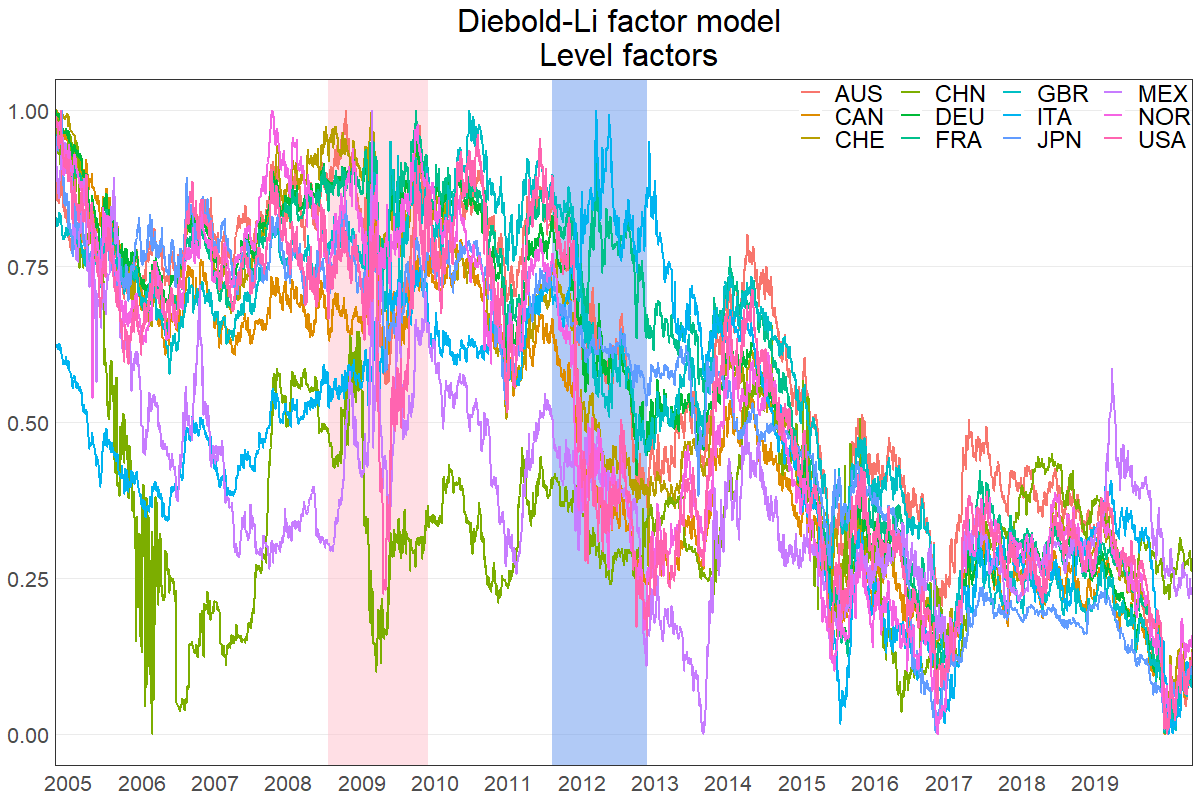
\includegraphics[width=\linewidth]{levels}
\caption{\textbf{Level}}

\end{subfigure}%
\begin{subfigure}{.5\linewidth}
\centering
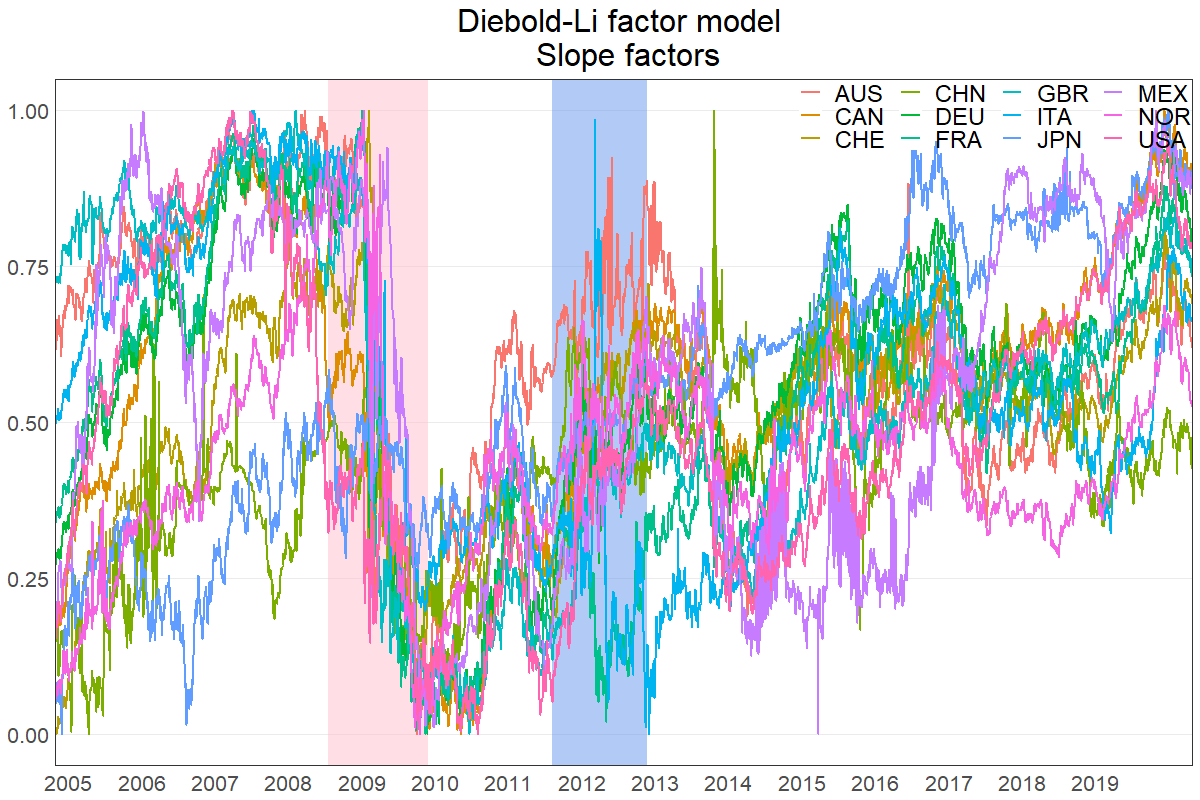
\includegraphics[width=\linewidth]{slopes}
\caption{\textbf{Slope}}
\end{subfigure}\\[1ex]
\begin{subfigure}{.5\linewidth}
\centering
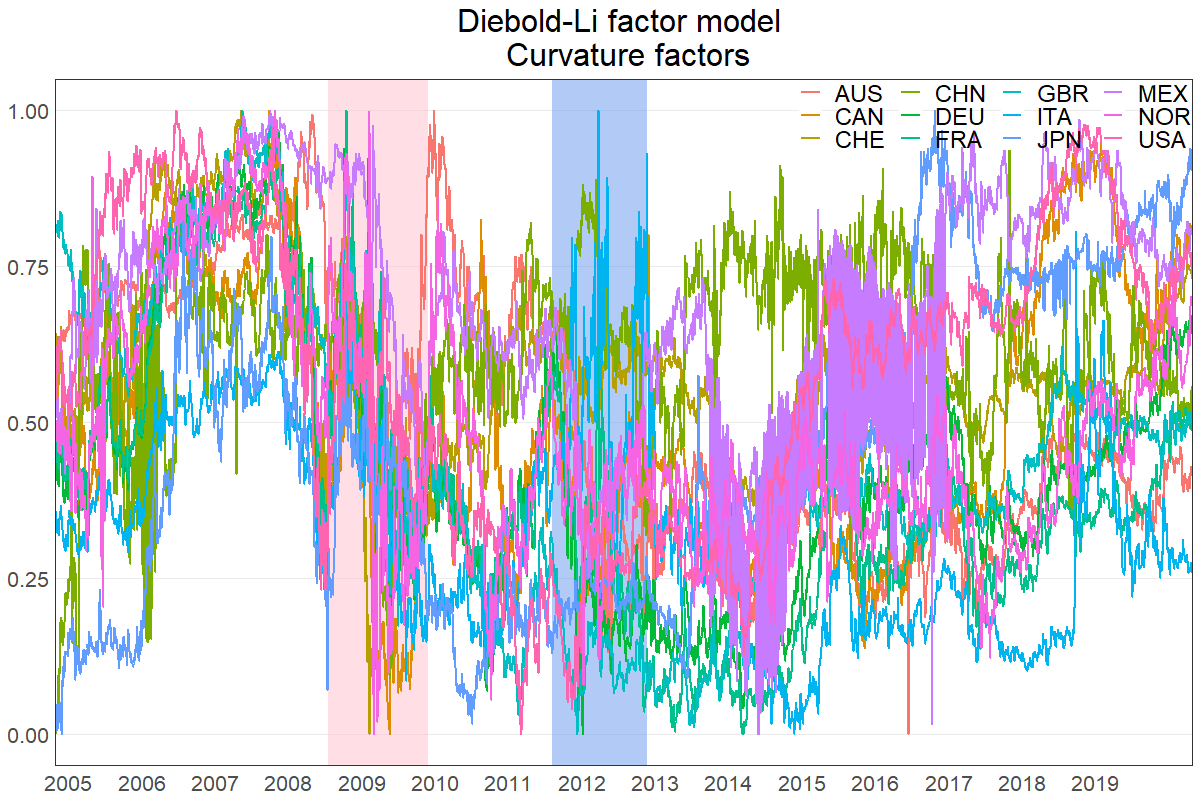
\includegraphics[width=\linewidth]{curvatures}

\caption{\textbf{Curvature}}
\end{subfigure}

\caption{Normlized factor time series}
\fnote{Start of the subprime crisis: J.P. Morgan takes over Bear Stearns, the troubled investment bank (03/16/08);

End of subprime crisis: 6/30/2009;

Start of the European sovereign debt crisis: Portuguese government calls on EU for bailout (04/06/11);

End of the European sovereign debt crisis: Draghi makes the famous ''Whatever It Takes'' speech (07/26/12).}

\end{figure}

%---------------------------------------------------------------------------------------------------------------------------------------------------------------------------

%\textcolor{red}{Es itt mondtad, hogy van egy eros faktorkomponens, arra egyelore nem nagyon tudok reagalni, azzal kapcsolatban mi lenne a tervunk?}

The descriptive statistics of the factors are represented in Table \textcolor{magenta}{1}. The average Level factor is positive in all cases, highest for Mexico and lowest for Japan. Average Slope refers to the tipical increasing shape of the yield curves (negative values). Slope is negative for all countries meaning that longer maturities have higher values than shorter ones. In absolute terms the USA has the highest Slope, while Australia has the lowest. Potential positive values of Slope represent restrictive monetary politics. Curvature is always negative too, highest for France and lowest for China (in absolute terms).


%-----------------------------------------------------------------------------------Table1-----------------------------------------------------------------------------
\begin{table}[H]

\fontsize{10}{10}\selectfont
\centering % used for centering table
\begin{tabular}{l c c c c c c}% centered columns (4 columns)
\hline\hline   \\ [-1.5ex]               %inserts double horizontal lines
%Case & Method\#1 & Method\#2 & Method\#3 & test \\  [0.5ex]
Factor & Average & Std. dev. & Minimum & Maximum & Jarque-Bera t-stat.  & P value \\ [0.5ex] % inserts table %heading

\hline       \\ [-1.5ex]           % inserts single horizontal line


\textit{\textbf{Germany}}		&		&		&		&		&		&		\\
Level						&	 2.92 &	1.54	&	-0.34	&	5.41	&	347	&	0.00	\\
Slope				&	-1.86	&	1.06	&	-4.54	&	0.14	&	210	&	0.00	\\
													
Curvature					&	-3.72	&	1.72	&	-7.15	&	0.73	&	234	&	0.00	\\
\textit{\textbf{Italy}}		&		&		&		&		&		&		\\
Level						&	4.78	&	1.29	&	1.98	&	8.00	&	106	&	0.00	\\
Slope				&	-3.43	&	1.57	&	-7.01	&	-0.44	&	183	&	0.00	\\
													
Curvature					&	-4.25	&	2.24	&	-8.60	&	4.75	&	194	&	0.00	\\
\textit{\textbf{France}}			&		&		&		&		&		&		\\
Level						&	3.39	&	1.37	&	0.26	&	5.48	&	417	&	0.00	\\
Slope				&	-2.24	&	1.19	&	-4.73	&	0.02	&	162	&	0.00	\\
													
Curvature					&	-4.29	&	1.96	&	-7.82	&	1.07	&	210	&	0.00	\\
\textit{\textbf{USA}}			&		&		&		&		&		&		\\
Level						&	3.96	&	0.99	&	1.88	&	5.87	&	323	&	0.00	\\
Slope				&	-2.41	&	1.55	&	-5.52	&	0.71	&	139	&	0.00	\\
													
Curvature					&	-3.63	&	2.50	&	-9.58	&	0.72	&	228	&	0.00	\\
\textit{\textbf{Canada}}				&		&		&		&		&		&		\\
Level						&	3.43	&	1.10	&	1.23	&	5.90	&	274	&	0.00	\\
Slope				&	-1.73	&	1.23	&	-4.84	&	0.58	&	251	&	0.00	\\
													
Curvature					&	-2.49	&	1.63	&	-6.26	&	1.31	&	206	&	0.00	\\
\textit{\textbf{Mexico}}			&		&		&		&		&		&		\\
Level						&	8.58	&	1.28	&	5.56	&	13.41&	834	&	0.00	\\
Slope				&	-2.36	&	1.83	&	-6.14	&	0.67	&	340	&	0.00	\\												
Curvature					&	-4.16	&	2.85&	-14.84&	0.49	&	321	&	0.00	\\
\textit{\textbf{Japan}}				&		&		&		&		&		&		\\
Level						&	1.70	&	0.83	&	-0.02	&	3.26	&	406	&	0.00	\\
Slope				&	-1.28	&	0.63	&	-2.83	&	-0.02	&	155	&	0.00	\\
													
Curvature					&	-3.69	&	1.28	&	-6.03	&	-0.87	&	278	&	0.00	\\
\textit{\textbf{China}}				&		&		&		&		&		&		\\
Level						&	4.02	&	0.62	&	2.70	&	6.52 &	2047	&	0.00	\\
Slope				&	-1.53	&	0.81	&	-3.87	&	1.65 &	275	&	0.00	\\
													
Curvature					&	-1.24	&	0.92	&	-5.20	&	1.25&	1128	&	0.00	\\
\textit{\textbf{Australia}}		&		&		&		&		&		&		\\
Level						&	4.63	&	1.23	&	1.40	&	6.77	&	262	&	0.00	\\
Slope				&	-0.89	&	0.98	&	-3.87	&	1.00	&	105	&	0.00	\\
													
Curvature					&	-2.08	&	1.84	&	-6.59	&	2.25	&	296	&	0.00	\\
\textit{\textbf{Norway}}				&		&		&		&		&		&		\\
Level						&	3.22	&	1.12	&	1.02	&	5.23	&	333	&	0.00	\\
Slope				&	-1.22	&	1.07	&	-4.04	&	2.26	&	167	&	0.00	\\
													
Curvature					&	-1.59	&	1.22	&	-4.68	&	1.73	&	337	&	0.00	\\
\textit{\textbf{United Kingdom}}		&		&		&		&		&		&		\\
Level						&	3.66	&	1.23	&	0.87	&	5.80	&	329	&	0.00	\\
Slope				&	-1.76	&	1.75	&	-5.42	&	1.35	&	211	&	0.00	\\
													
Curvature					&	-3.33	&	3.02	&	-8.77	&	3.65	&	159	&	0.00	\\
\textit{\textbf{Switzerland}}				&		&		&		&		&		&		\\
Level						&	1.77	&	1.18	&	-0.76	&	3.86	&	289	&	0.00	\\
Slope				&	-1.18	&	0.70	&	-3.32	&	0.91	&	219	&	0.00	\\
Curvature					&	-2.94	&	1.21	&	-7.77	&	0.62	&	543	&	0.00	\\

\hline%inserts single line
\end{tabular}
\label{table:nonlin}% is used to refer this table in the text

\caption{Descriptive statistics of yield curve factors}% title of Table
\end{table}
%----------------------------------------------------------------------------------------------------------------------------------------------------

%------------------------------------------------ table2---------------------------------------------------------------------------------

\bigskip


Factor time sereies are tested with (\cite{bera1981efficient}) test for normality. Neither of them passes the acceptance criteria therefore the null-hypothesis for normaility is rejected. Furthermore ADF and KPSS unit-root tests for stationarity are applied. Curvature for China and Slope for Japan is stationary on the usual 95\% confidence level. The tests can be applied for first differenence of the remaining time series too. The unit-root test results are represented in Table \textcolor{magenta}{5} in the Appendix.

Before differentiating, a pairwise  (\cite{engle1987co} test is applied for determining cointegrations. Table \textcolor{magenta}{2} represents the ratio of the cointegrated time series aggregated by factors. Besides the diagonal, the Slope - Curvature and the Curvature - Slope pairs both show a value more than 70\%. Since the time series are not stationary on the same order and the ratio of cointegrated time series is high, we consider the Toda-Yamamoto approach to be justified for analyzing connections.

%--------------------------------------------------------------------------------Table3 -------------------------------------------------------
\begin{table}[H]


\centering% centering table
\begin{tabular}{l | ccc}% creating eight columns
\hline\hline \\ [-1.5ex]                         %inserting double-line

	&	Level 	&	Slope	&	Curvature	\\
\hline \\ [-1.5ex]  
Level	&	75.7\%	&	44.4\%	&	64.6\%	\\
Slope	&	29.2\%	&	74.3\%	&	71.5\%	\\
Curvature	&	29.2\%	&	78.5\%	&	75.0\%	\\


\hline            





\end{tabular}
\label{table:nonlin}% is used to refer this table in the text
\caption{Pairwise Engle-Granger test} %title of the table
\end{table}

    \begin{tablenotes}
      \small
     \item \centering \textit{Instead of the 36 x 36 matrix which we obtain from the pairwise Engle-Granger test, we highlight only the factor-wise aggregated values in this table.}
    \end{tablenotes}

%----------------------------------------------------------------------------------------------------------------------------------------------------



\section{Results}

\subsection{Static interconnectedness}

%A Toda-Yamamoto módszerrel kapott összekötöttségi hálózatokat statikus és dinamikus szemlélet szerint is elemzem. A statikus modellbe a rendelkezésre álló összes adatpont bekerült. Az idősorokat maximum egyszer differenciázom, a modellhez szükséges optimális késleltetési szintet pedig az AIC alapján határozom meg. Az 1\%-os szignifikancia szint mellett a modellből nyert oksági kapcsolatokat a 3. ábra mutatja. A Szint faktorokat pirossal, a Meredekséget kékkel, a Görbületet zölddel jelölöm. A két faktor közötti nyíl az okság irányát mutatja, a színe pedig arra a faktorra utal, amelyikből kiindult.

We perform static and dynamic analysis of the factor interconnectedness resulted by the Toda-Yamamoto model. All of the available data points are used in the static method. Time series are differenciated once at maximum, and the optimal lag number is determined based on AIC. Figure textcolor{magenta}{2} shows the causailiy relationships on 1 \% sigificance level. Level factors are red, while Slope is blue and the Curvature is showed in green. The arrow between two factors shows the direction of the causality and its color represent the factor which it is started from.

%A három alrendszerből a legsűrűbbnek a Meredekségek hálózata bizonyul. A potenciális kapcsolatok 31.06\%-a szignifikáns. Ezt követi a Szint (21.97\%) majd a Görbület (17.42\%). A keresztkapcsolatokat tekintve, az összes Szint faktorból kimenő lehetséges élek 31.25\%-a szignifikáns, a Meredekségeknél ez az arányszám 26.39\%, míg a Görbület ilyen értelemben is a legkevésbé összekötött faktor, a kimenő élek 20.49\%-a szignifikáns.

From the three subsystems, the Slope network is the most dense. 31.06\% of the potential relationships is significant. It is followed by Level (21.97\%), then Curvature (17.42\%). Considering cross connections, 31.25\% of the possible edges going out from Level factors is significant. This ratio is 26.39\% for Slope, and Curvature is the least interconnected factor in these terms, only 24.49\% of the outgoing edges is significant.


%--------------------------------------------------------------------------------Fig3 -------------------------------------------------------
\begin{figure}[H]

  \begin{subfigure}[t]{.5\textwidth}
    \centering
    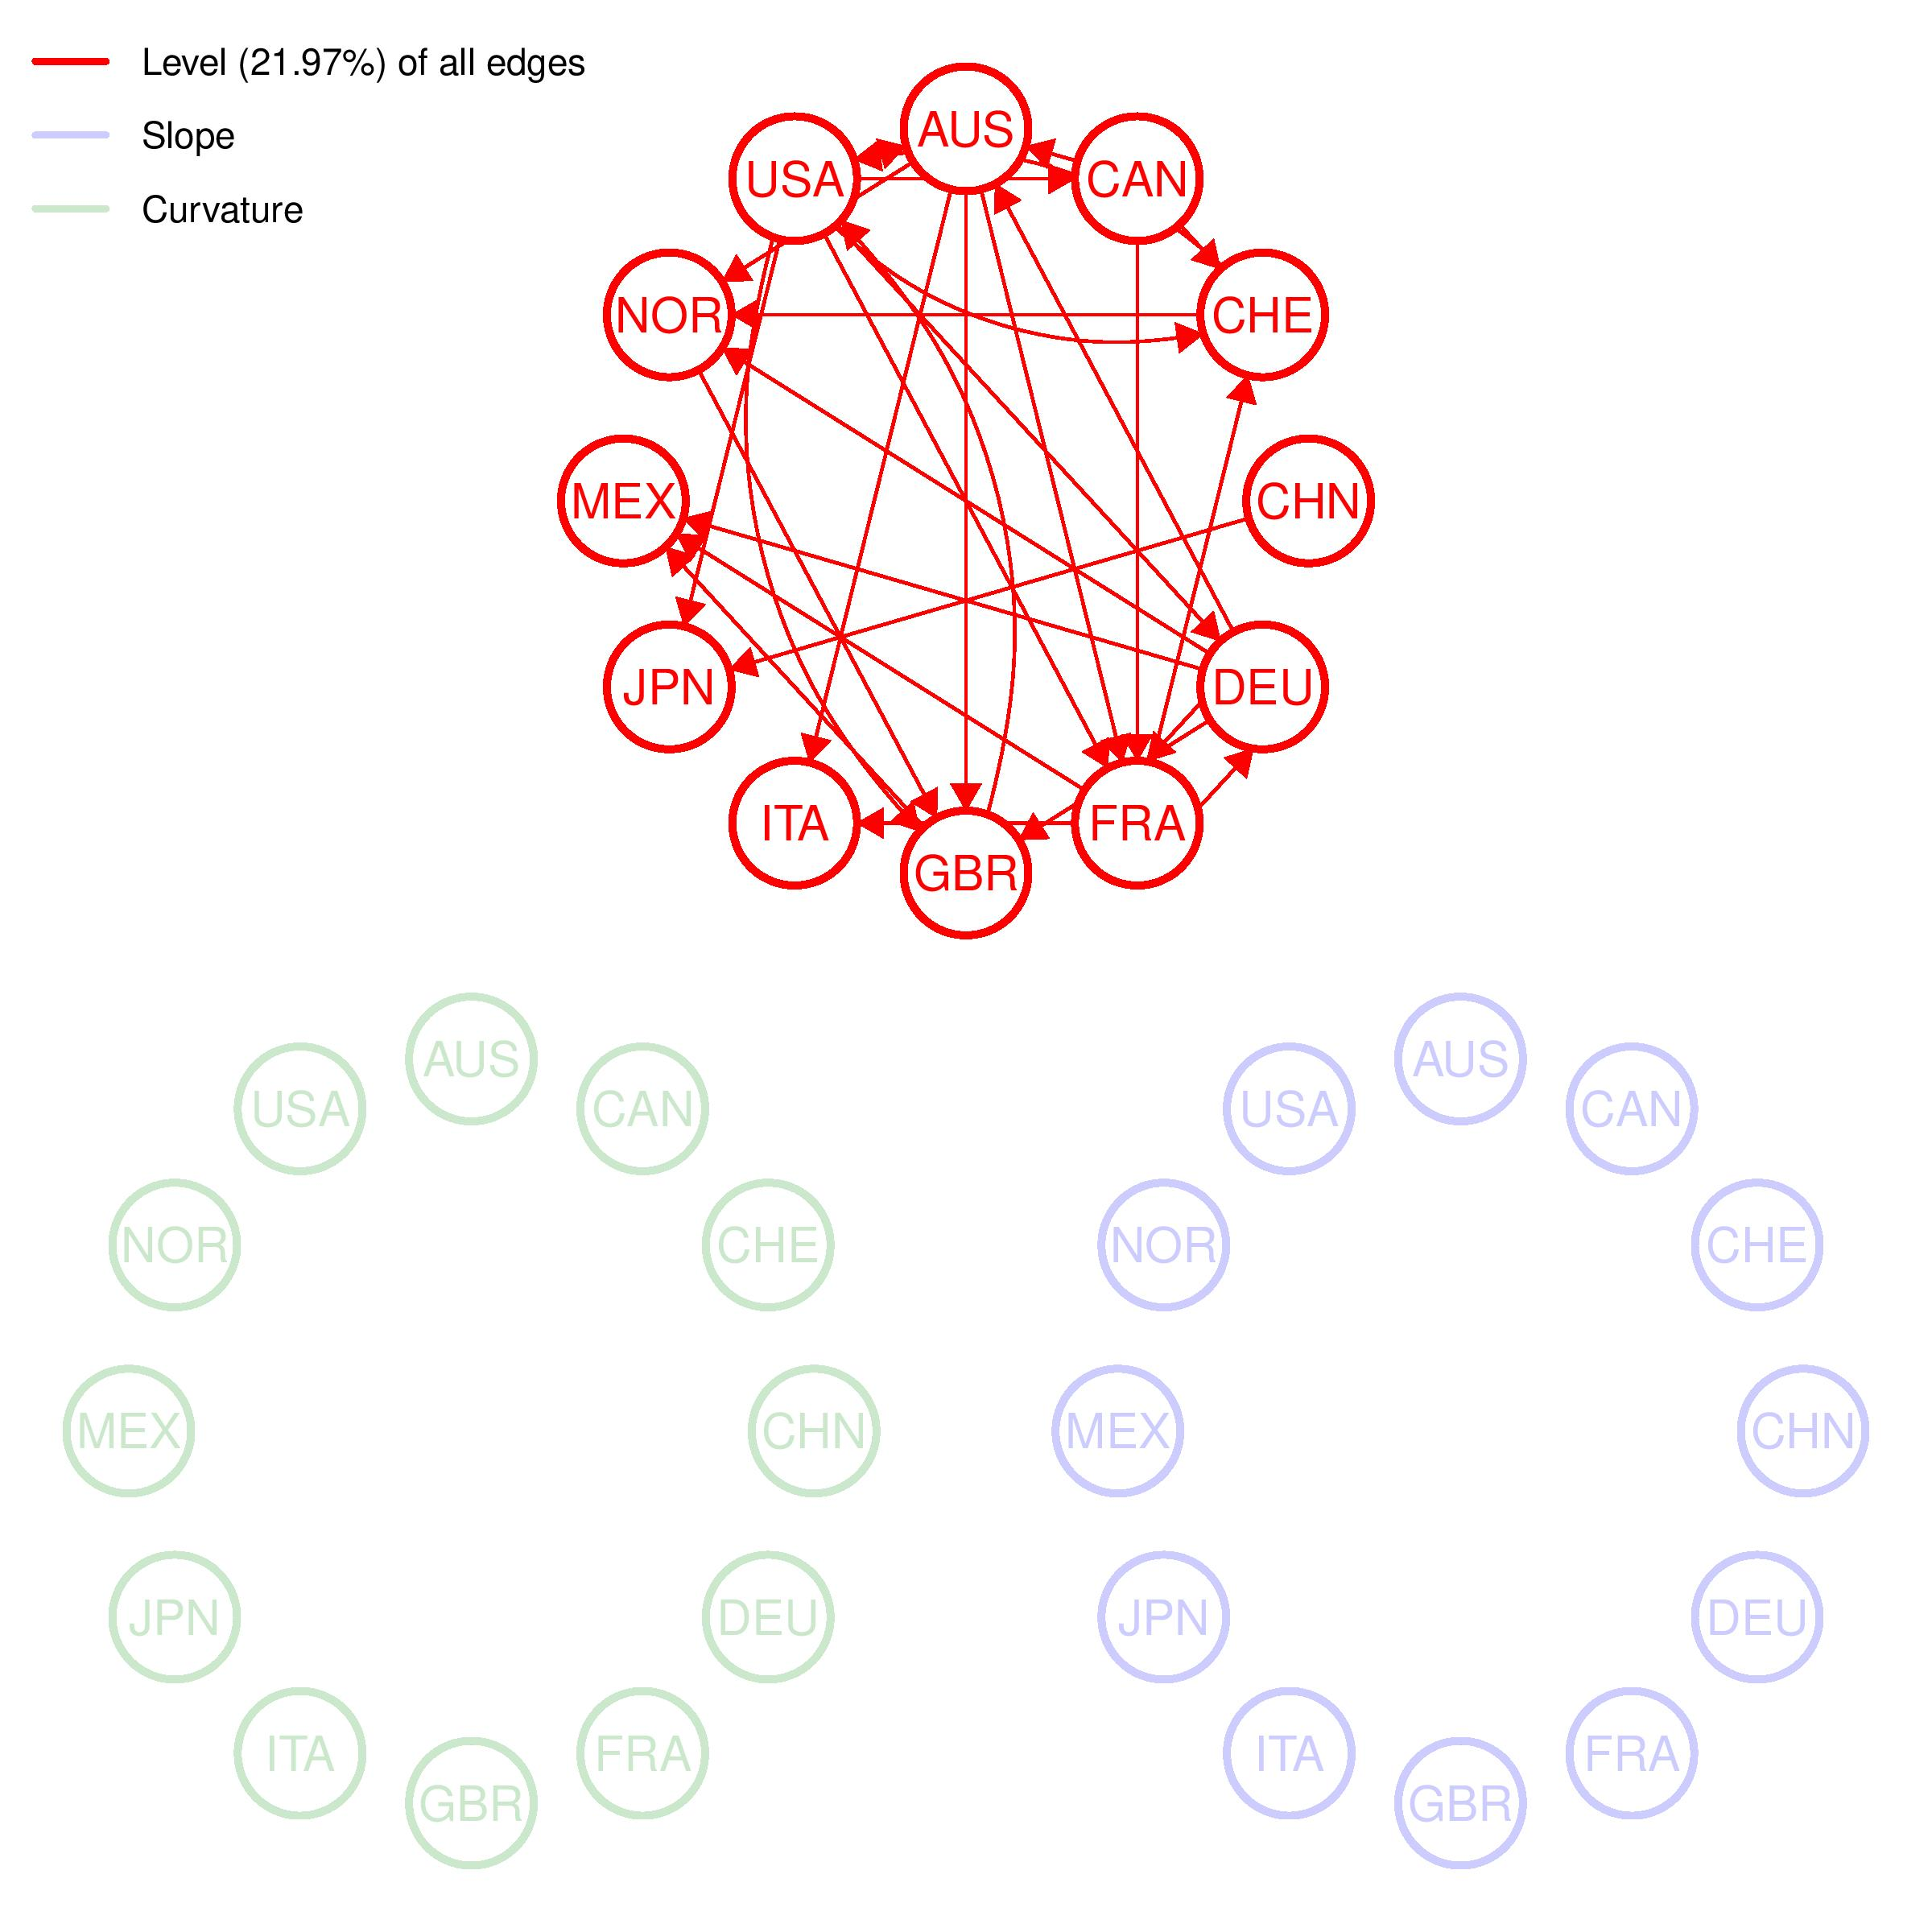
\includegraphics[width=\linewidth]{All_plot_onlylevel2004-07-01_2019-12-31_0.01-page-001}
    \caption{\textbf{Level subnetwork}}
  \end{subfigure}
  \hfill
  \begin{subfigure}[t]{.5\textwidth}
    \centering
    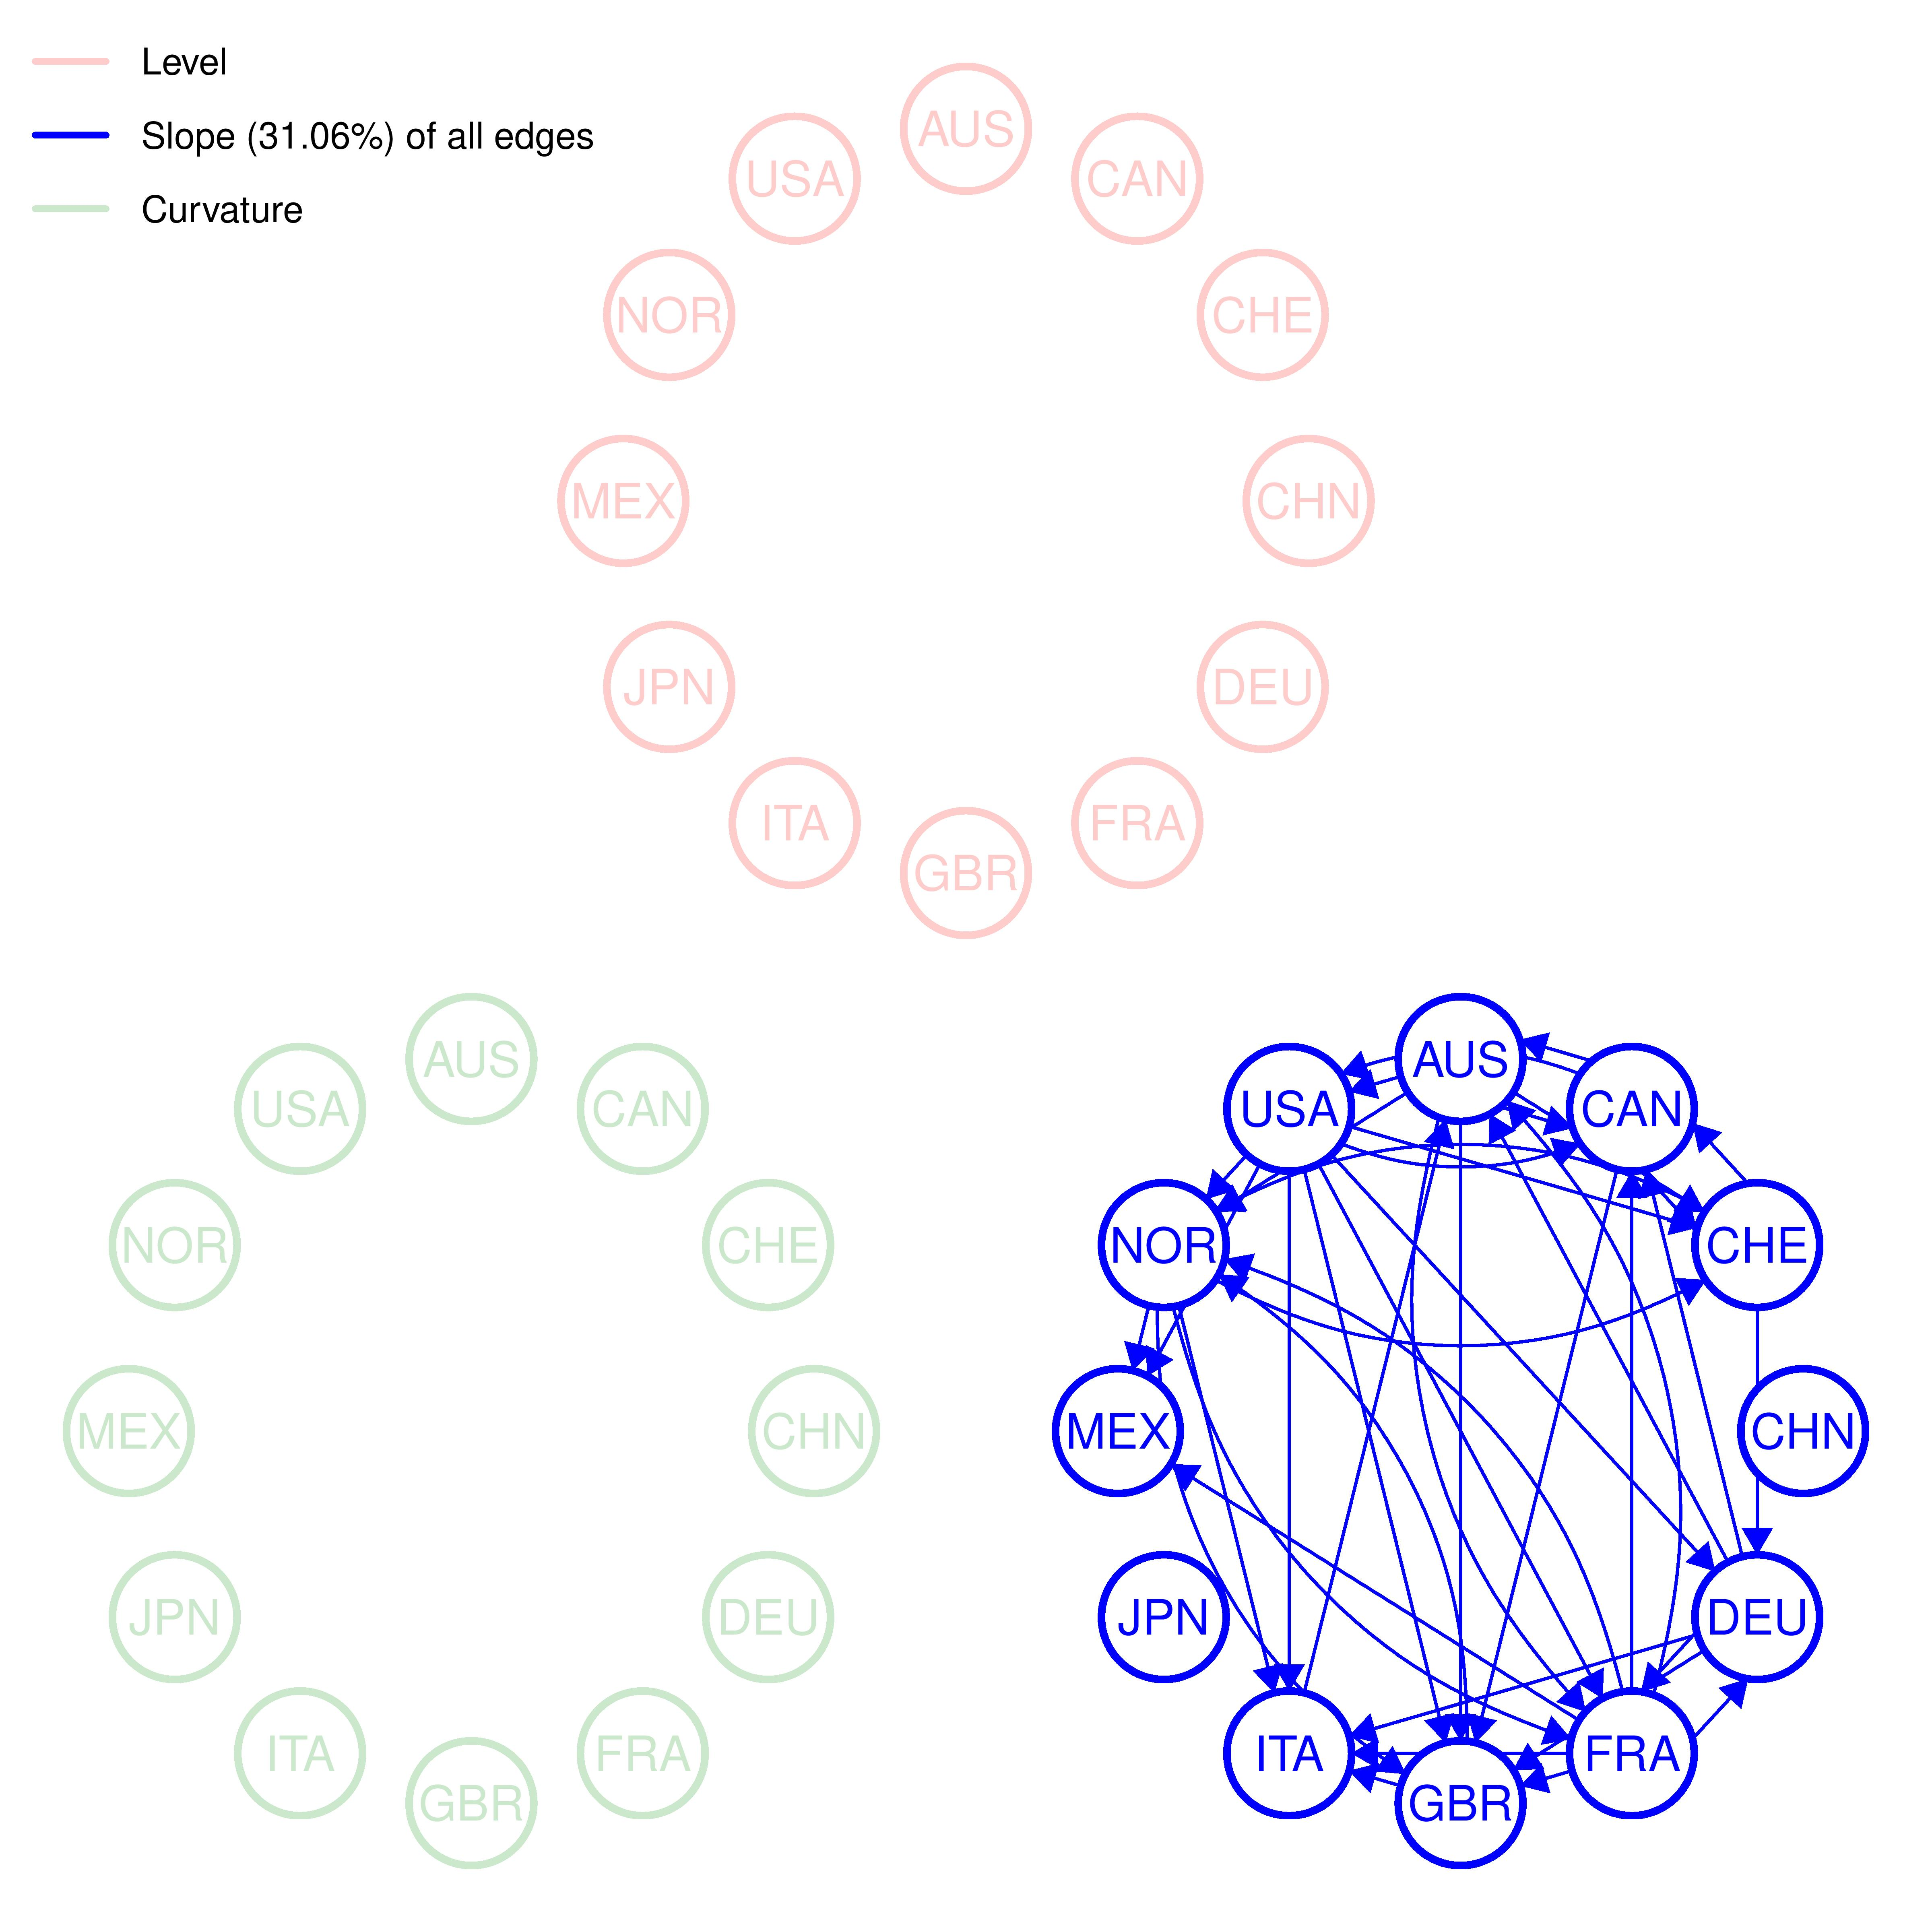
\includegraphics[width=\linewidth]{All_plot_onlyslope_2004-07-01_2019-12-31_0.01-page-001}
    \caption{\textbf{Slope subnetwork}}
  \end{subfigure}

  \medskip

  \begin{subfigure}[t]{.5\textwidth}
    \centering
    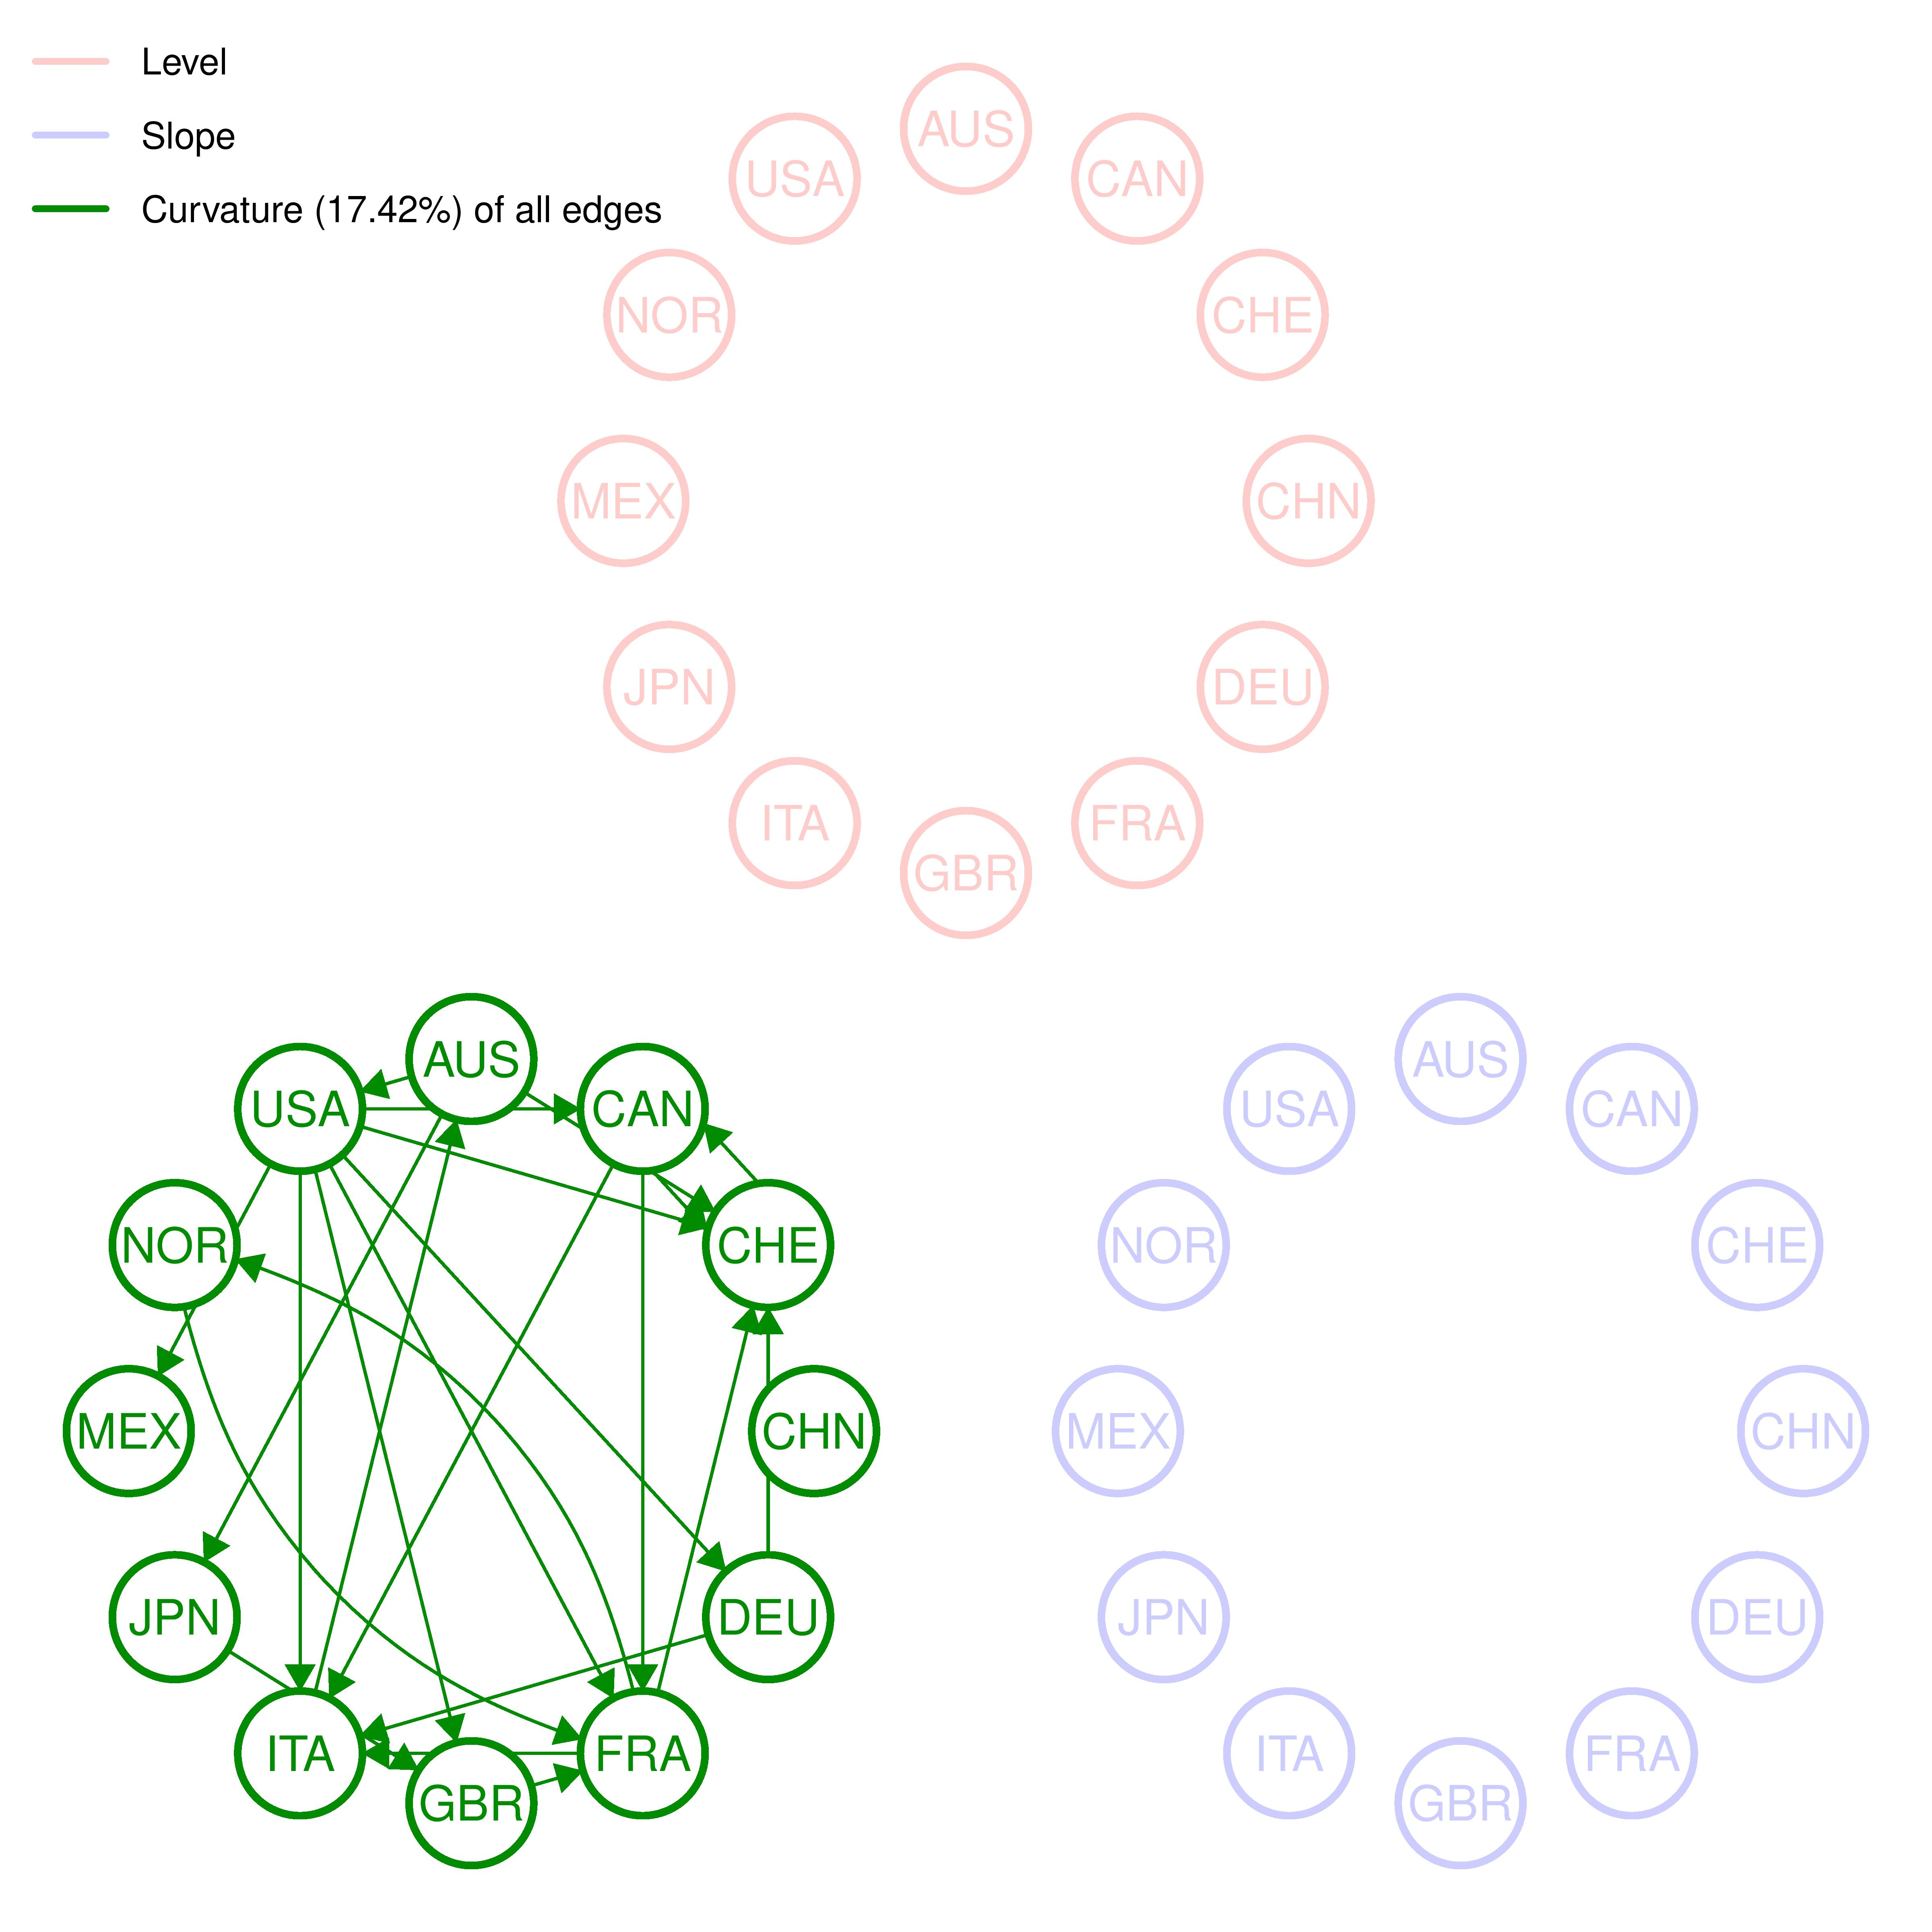
\includegraphics[width=\linewidth]{All_plot_onlycurv_2004-07-01_2019-12-31_0.01-page-001}
    \caption{\textbf{Curvature subnetwork}}
  \end{subfigure}
  \hfill
  \begin{subfigure}[t]{.5\textwidth}
    \centering
    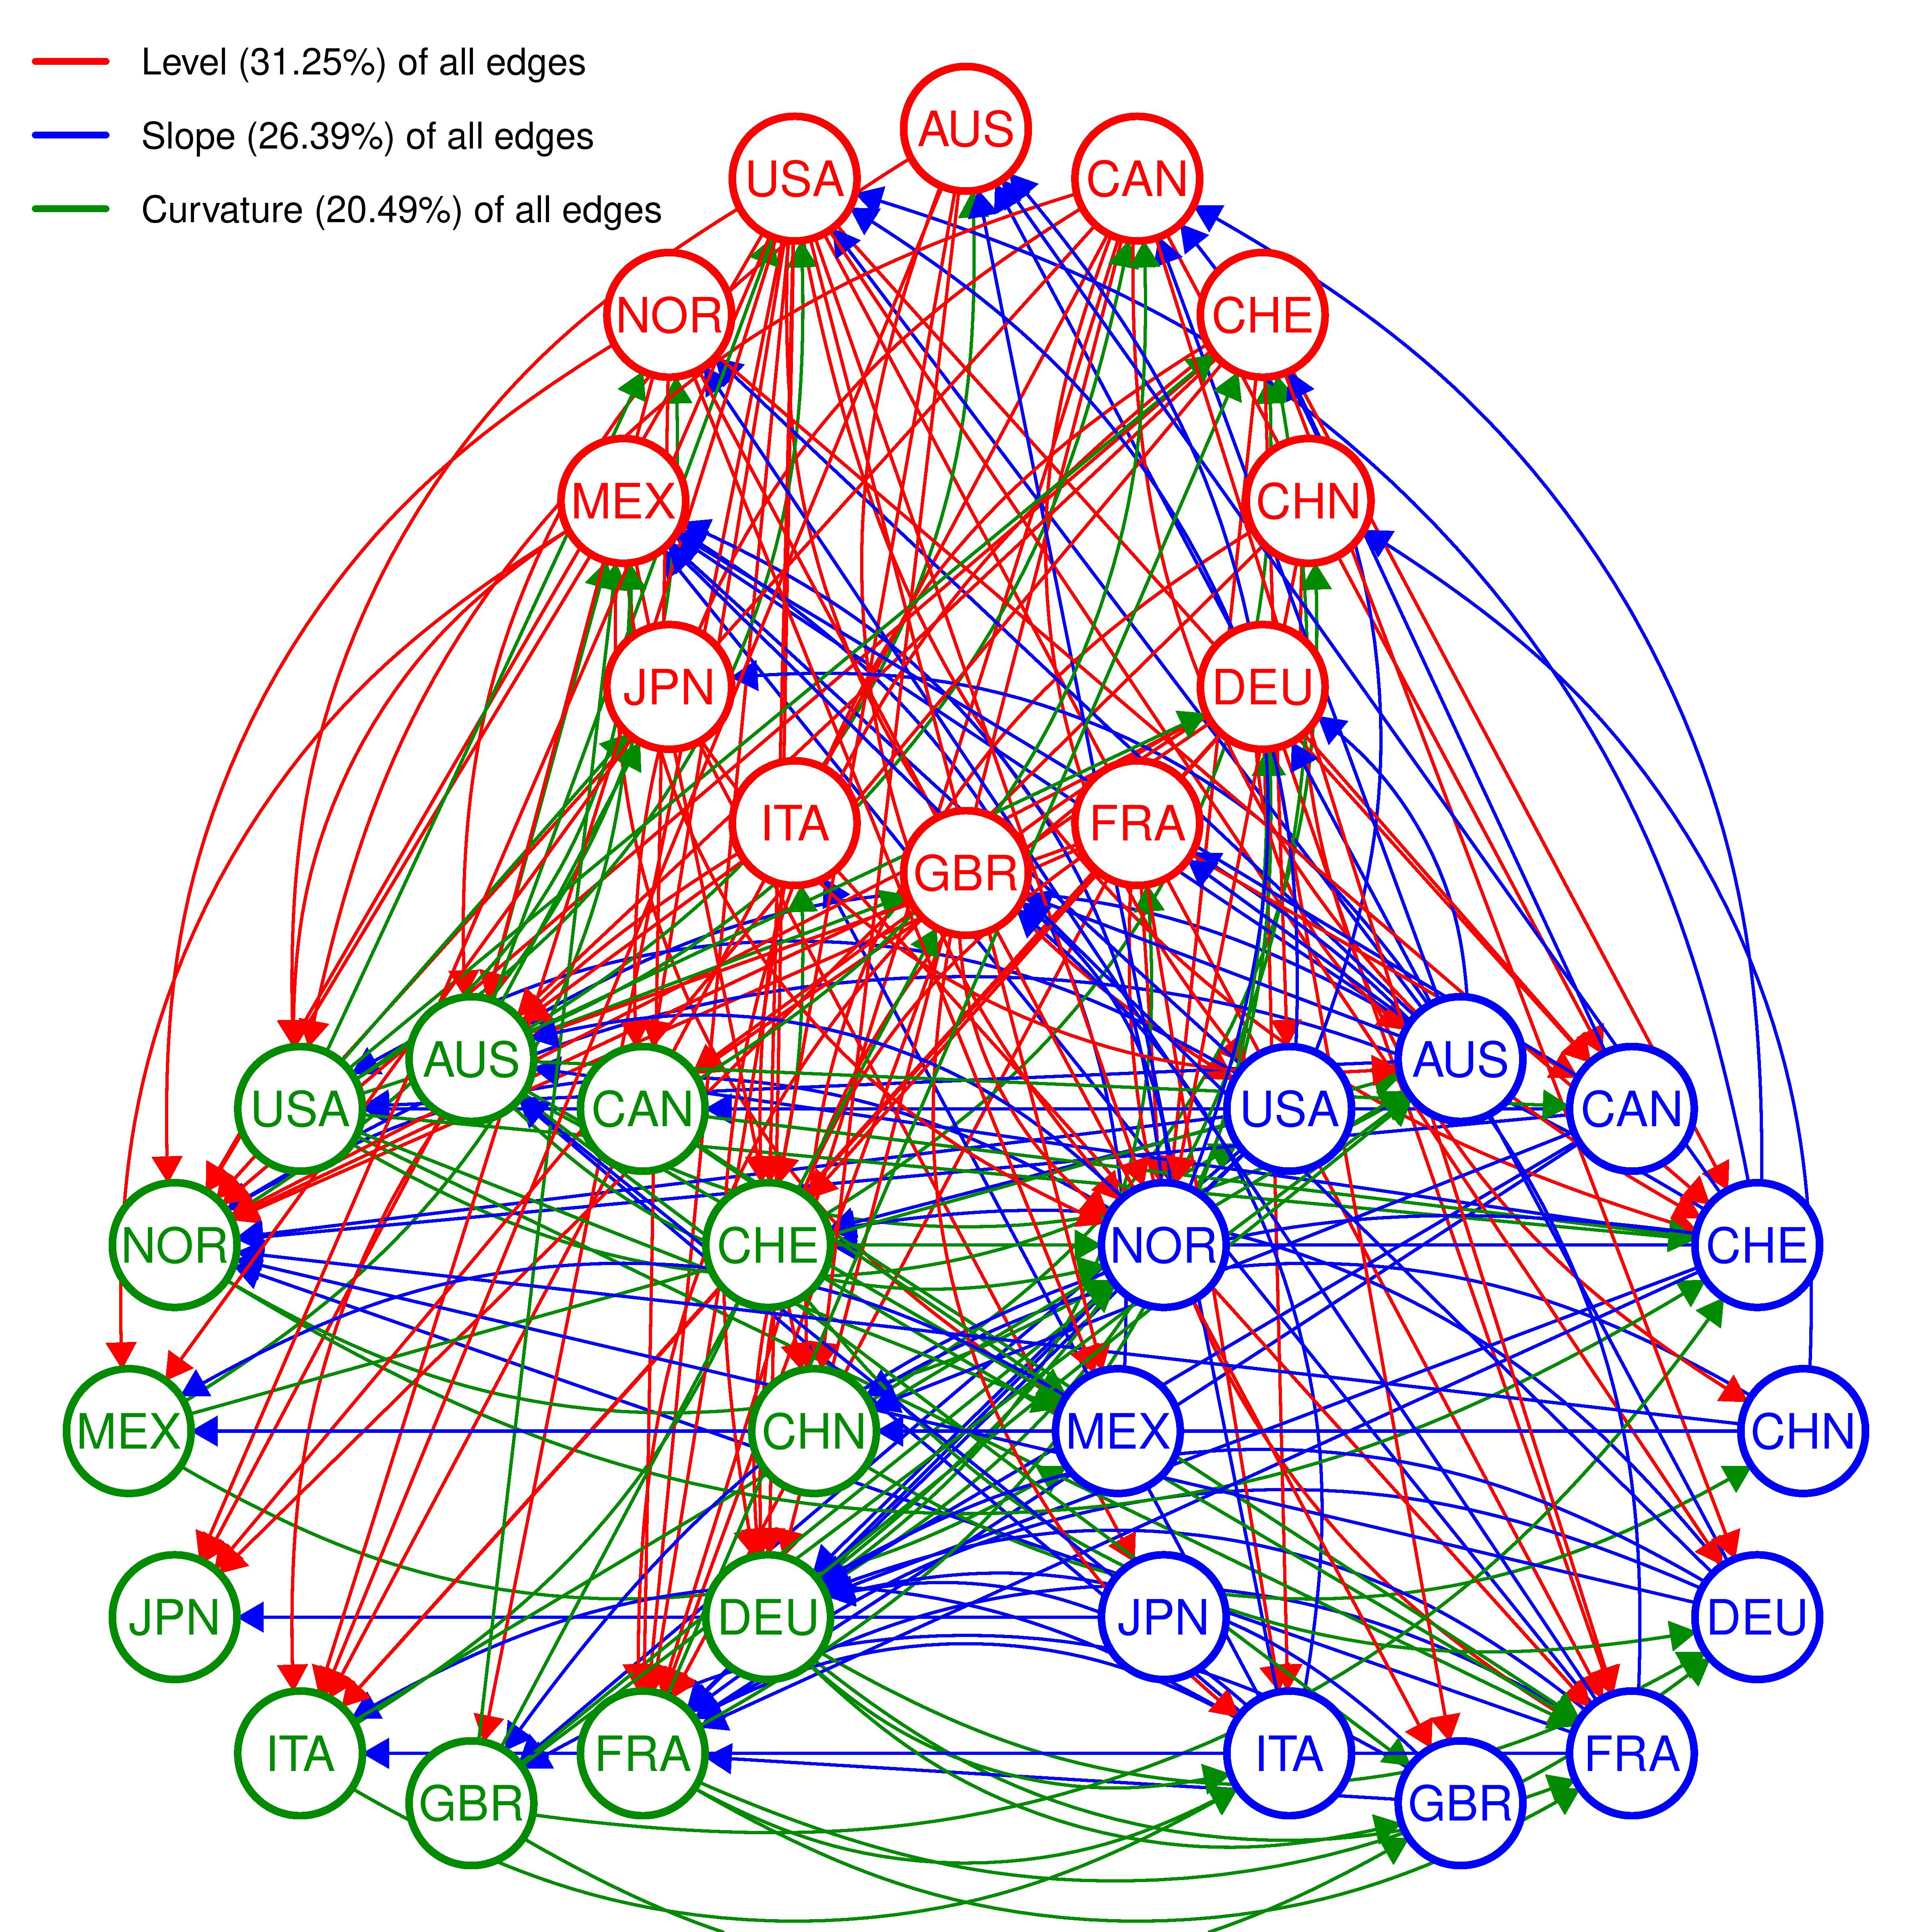
\includegraphics[width=\linewidth]{All_plot_innerempty_2004-07-01_2019-12-31_0.01-page-001}
    \caption{\textbf{Cross connections}}
  \end{subfigure}
  \caption{Interconnectedness in subnetworks}
\end{figure}

%----------------------------------------------------------------------------------------------------------------------------------------------------

\bigskip

%A 4. táblázat (a) része tartalmazza a rendszerben definiált élek számát. A táblázat sorai a kapcsolatok eredetét mutatják, az oszlopok pedig a nyilak végpontjaira utalnak. 1\%-os szignifikancia szinten, a gráfnak 318 éle van, ami az összes lehetséges élnek a 25.24\%-a. A 4. táblázat (b) része tartalmazza az alrendszerek között definiált élek arányát, az abban a viszonyrendszerben értelmezett maximális kapcsolatok számához képest. Ezek alapján elmondható, hogy a Szint és Görbület közötti okság a legsűrűbb, 36.1\%, ezt követi a Meredekség és Görbület közötti összekö-töttség, 31.94\%-kal, a harmadik helyen pedig a Szint alhálózat alatt értelmezett nyilak aránya áll, 31.06\%-kal. A kapcsolati mátrix nem szimmetrikus a főátlóra, a Görbület faktorokból, összesítve kevesebb nyíl irányul mind az alhálózaton belülre, mind kívülre.

The (a) part of Table \textcolor{magenta}{4} contains the number of edges defined in the system. Rows of the table represent the origin of the relationship, while columns stand for the endpoints of the arrows. On 1\% significance level, the graph has 318 edges which is 25.24\% of the total potential edges. (b) part of Table \textcolor{magenta}{4} shows the ratio of the edges defined within subnetworks compared to the total potential edges definable in that given relationship system. Based on this, density of causality is the highest for Level - Curvature pair, 36.1\% followed by Slope - Curvature which is 31.94\%. The third place goes for the Level subnetork with 31.06\%. The relationship matrix is symmetrical for the diagonal, in total from the Curvature factor there is less arrows going out both internally and towards other subnetworks.

%--------------------------------------------------------------------------Table4--------------------------------------------------------------------------


\begin{table}[H]

\fontsize{9}{9}\selectfont
\centering
\begin{subtable}[t]{0.35\textwidth}
\centering
\begin{tabular}{l | ccc  r}% creating eight columns
\hline\hline \\ [-1.5ex]                         %inserting double-line

	&	Level 	&	Slope	&	Curvature	& Sum  \\ 
\hline \\ [-1.5ex]  
Level	&	29	&	38	&	52	&	119 	\\
Slope	&	30	&	41	&	46	&	117	\\
Curvature	&	25	&	34	&	23	&	82	\\
\hline \\ [-1.5ex]  
Sum	&	84	&	113	&	121	&	318	\\


\hline            
\end{tabular}
\caption{\textbf{Number of edges, grouped by factors}}
%\label{table:nonlin}% is used to refer this table in the text
\end{subtable}
\hspace{\fill}
\begin{subtable}[t]{0.5\textwidth}
\centering
\begin{tabular}{l | ccc  r}% creating eight columns
\hline\hline \\ [-1.5ex]                         %inserting double-line



	&	Level	&	Slope	&	Curvature	&	Sum.	\\
\hline \\ [-1.5ex] 
Level	&	22.0\%	&	26.4\%	&	36.1\%	&	84.5\%	\\
Slope	&	20.8\%	&	31.1\%	&	31.9\%	&	83.8\%	\\
Curvature	&17.4\%	&	23.6\%	&	17.4\%	&	58.4\%	\\
\hline \\ [-1.5ex]  
Sum.	&	60.2\%	&	81.1\%	&	85.5\%	&	25.2\%	\\
\hline  
\end{tabular}
\caption{\textbf{Distribution of edges, grouped by factors}}
%\label{table:nonlin}% is used to refer this table in the text
\end{subtable}
\caption{The number and distibution of the sygnificant edges defined in the system} %title of the table
\end{table}
%----------------------------------------------------------------------------------------------------------------------------------------------------

\subsubsection{Top nodes}

Table \textcolor{magenta}{5} contains the factors with the most edges. The first quarter of the list stands for the summarized relationships, then the following columns represent the nodes having the most incoming and outgoing edges separatedly. In total, Level factor of the United States has the most edges, which is 30. Fom this 30, there are 23 outgoing and 7 incoming arrows. This relationship system is shown on Figure \textcolor{magenta}{5}. Generally speaking, all three factors of the USA leads the list regarding both outgoing and net (outgoing-incoming) edges. This can be interpreted as the USA has a high affecting power on the values of the factors of the remaining participants in the system and in the meanwhile it is not affected by the others. In the list of outgoing edges, Curvature of Asutralia is ahead of the Level of Germany which node is on the fourth place of the net chart, before the Level of Canada. The most causality effect is arriving towards the French Curvature followed by the Italian Slope, then the Curvature of the same country.

%--------------------------------------------------------------------------Table5--------------------------------------------------------------------------
\begin{table}[h]

\fontsize{10}{10}\selectfont
\setlength{\tabcolsep}{10pt}
\centering% centering table
\begin{tabular}{l  lcc  lc lc  lc}% creating eight columns

\hline\hline \\ [-1.5ex]                         %inserting double-line


\multicolumn{4}{c}{Top 5 Sum}					&	\multicolumn{2}{c}{Top 5 Incoming}			&	\multicolumn{2}{c}{Top 5 Outgoing}			&	\multicolumn{2}{c}{Top 5 Net}	\\	
\hline \\ [-1.5ex]    
Node	&	Total 	&	In	&	Out	&	Node	&	In	&	Node	&	Out	&	Node	&	Net	\\
\hline \\ [-1.5ex]    
USA\_L&	30	&	7	&	23	&	FRA\_C	&	19	&	USA\_L	&	23	&	USA\_L	&	16	\\
AUS\_S	&	28	&	11	&	17	&	ITA\_S	&	16	&	USA\_S	&	18	&	USA\_S	&	12	\\
FRA\_S	&	28	&	14	&	14	&	ITA\_C	&	16	&	USA\_C	&	17	&	USA\_C	&	10	\\
NOR\_S	&	27	&	16	&	11	&	MEX\_L	&	14	&	AUS\_S	&	17	&	DEU\_L	&	9	\\
FRA\_C	&	27	&	19	&	8	&	FRA\_S	&	14	&	DEU\_L	&	16	&	CAN\_L	&	7	\\

\hline            
\end{tabular}
\label{table:nonlin}% is used to refer this table in the text

\caption{Factors having most edges} %title of the table

\end{table}


%----------------------------------------------------------------------------------------------------------------------------------------------------



%--------------------------------------------------------------------------Fig4--------------------------------------------------------------------------
\begin{figure}[H]

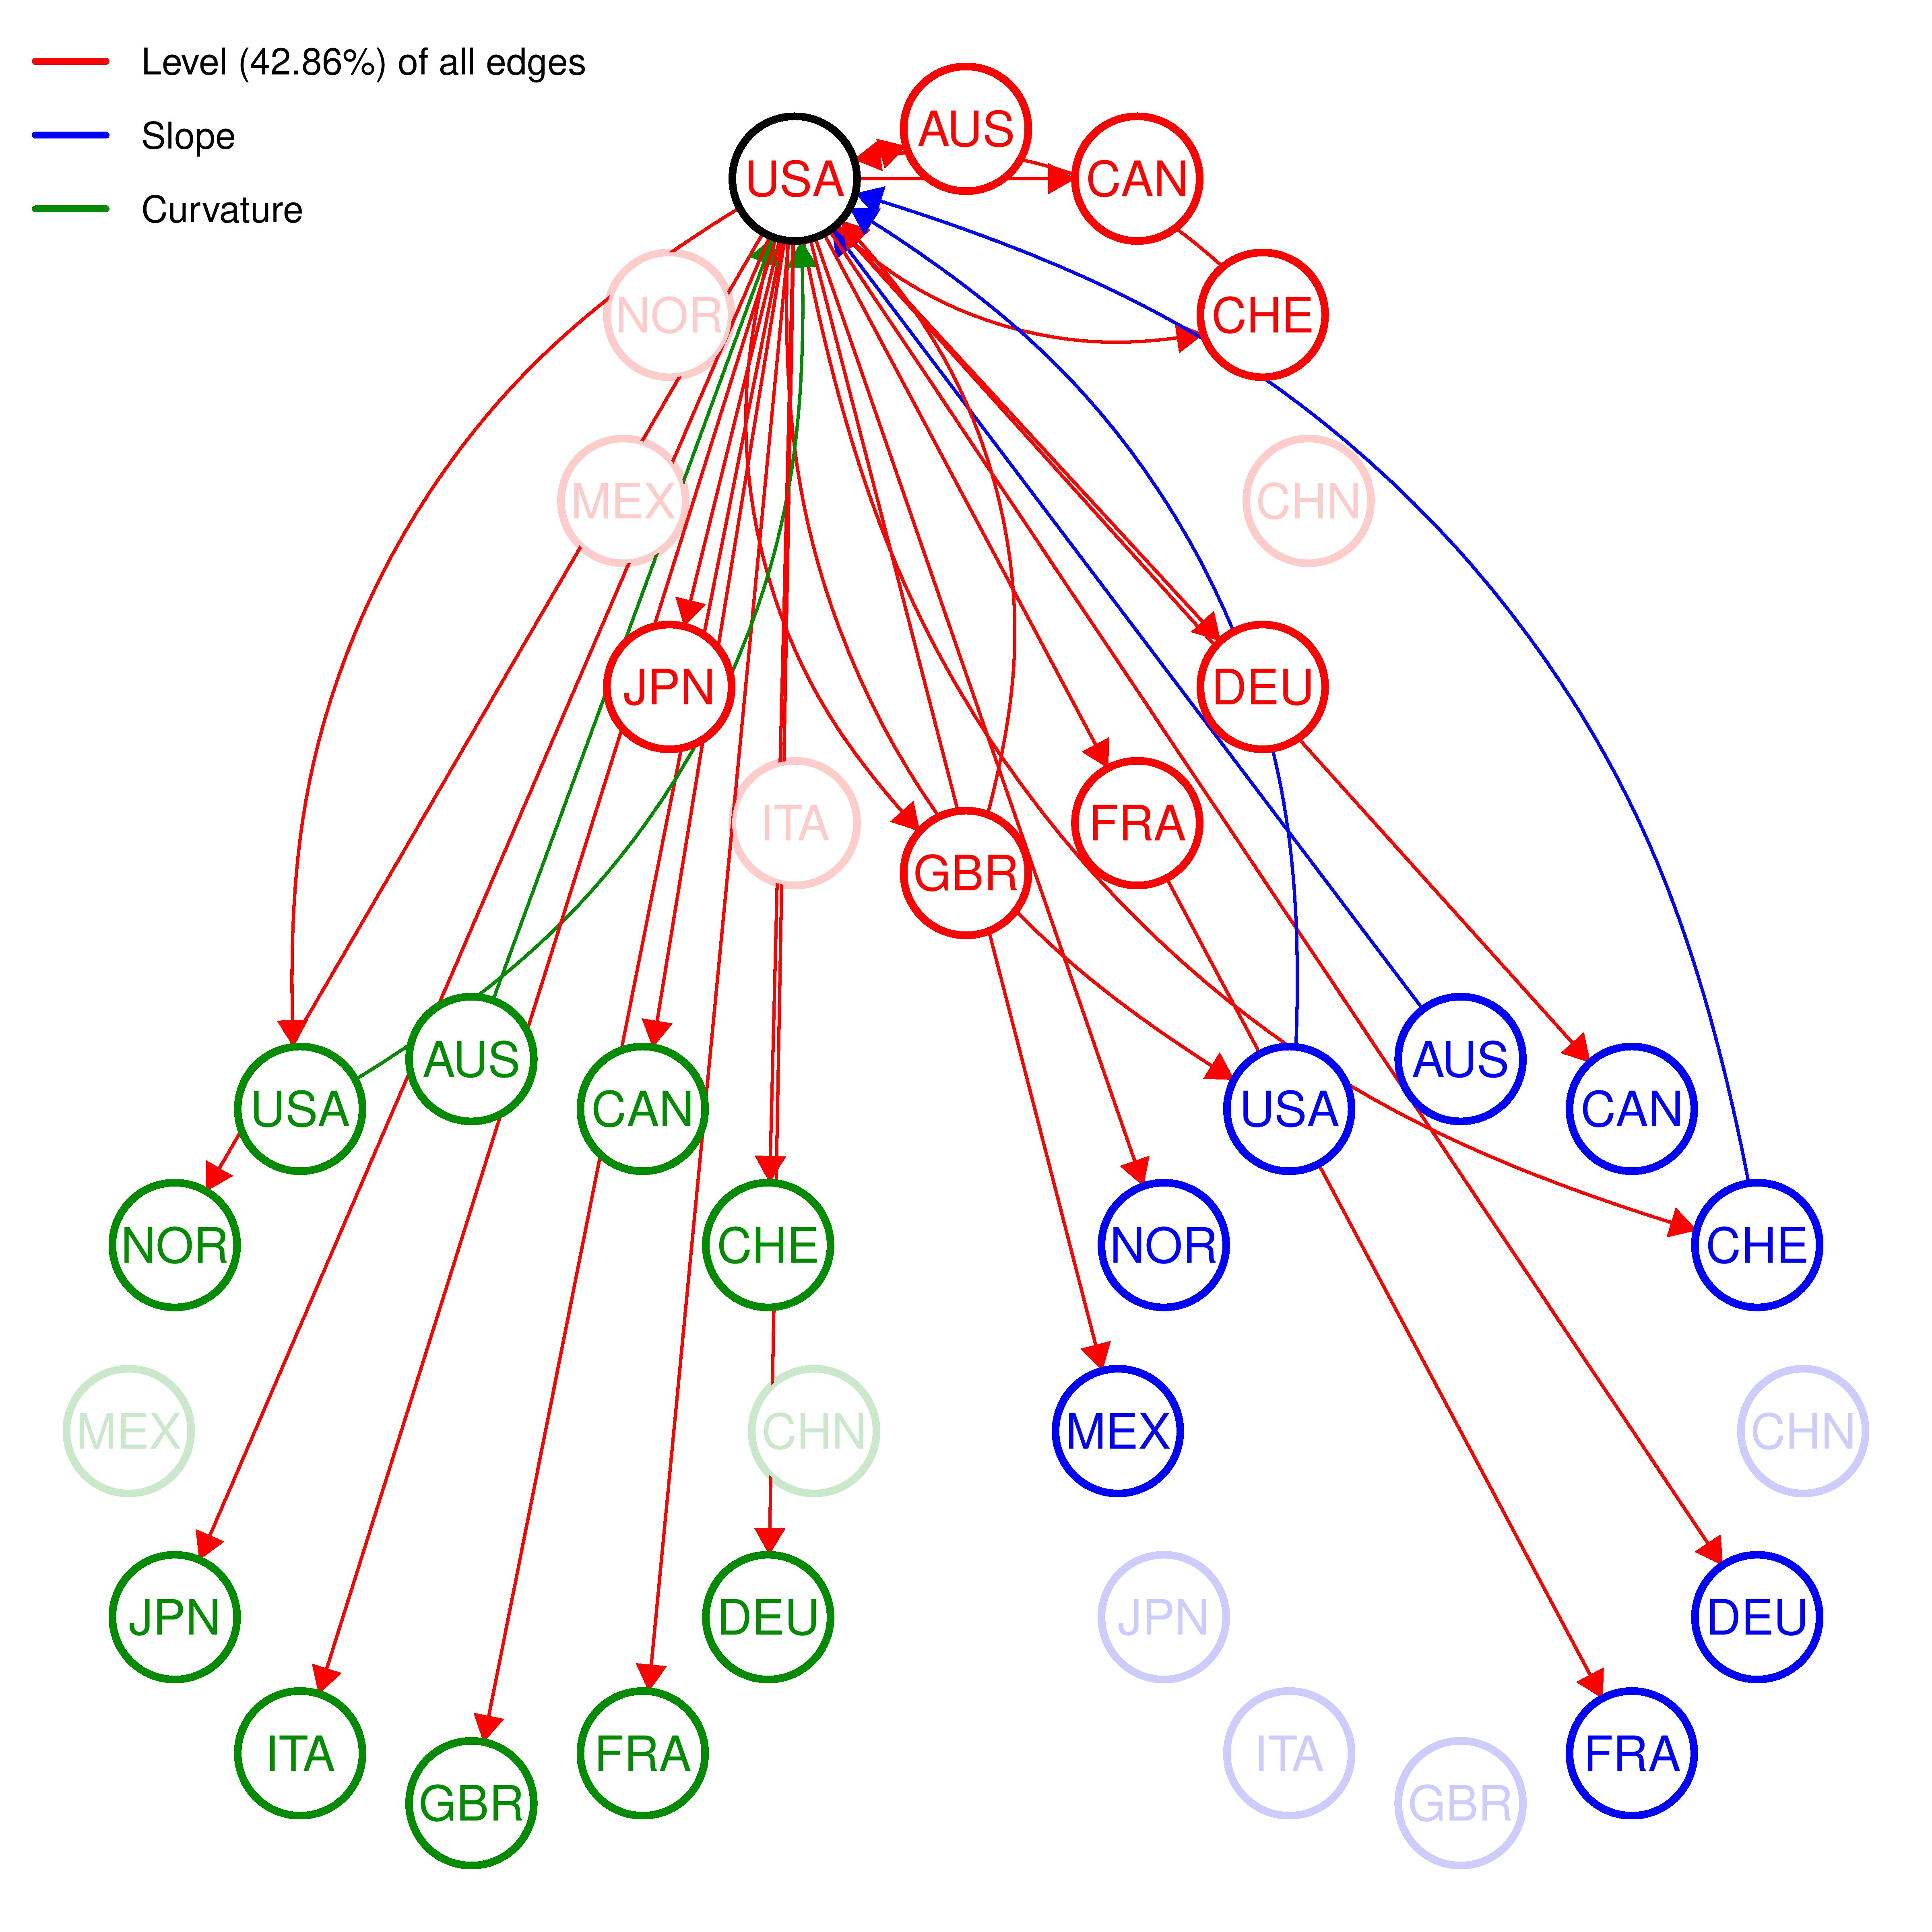
\includegraphics[width=13.5cm]{USA_B_1_plot_2004-07-01_2019-12-31_0.01-page-001}
\centering
\caption{Node having most summarized edges}

\end{figure}

\begin{figure}[H]

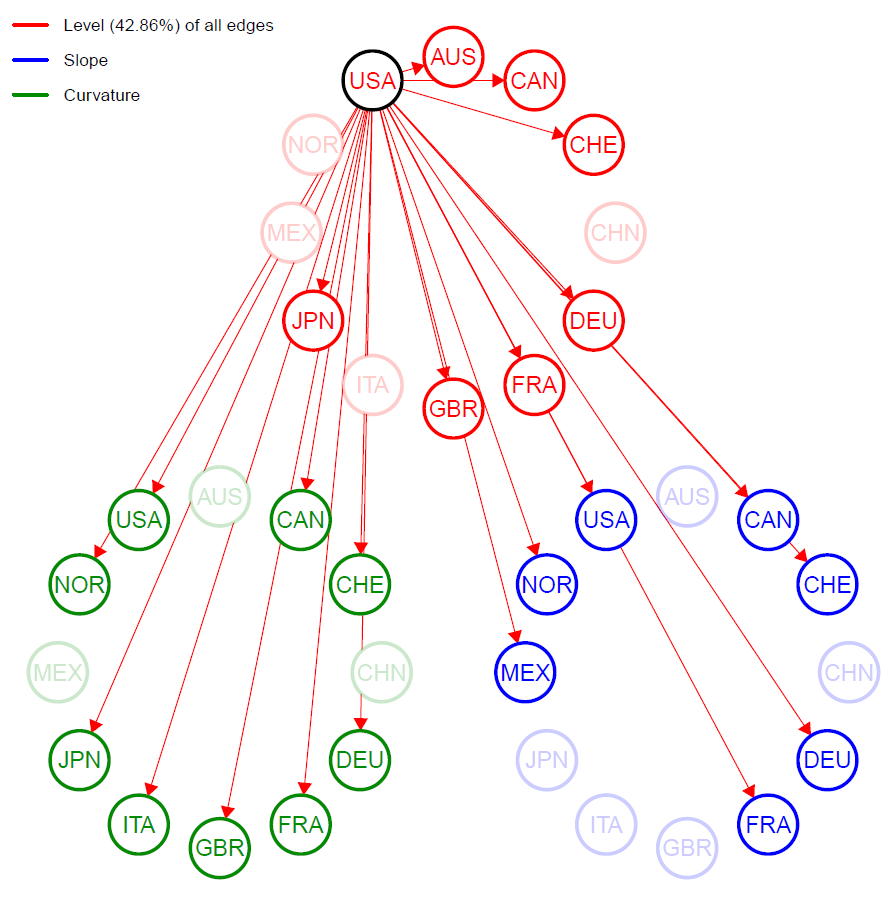
\includegraphics[width=13.5cm]{top_out}
\centering
\caption{Node having most outgoing edges}

\end{figure}

\begin{figure}[H]

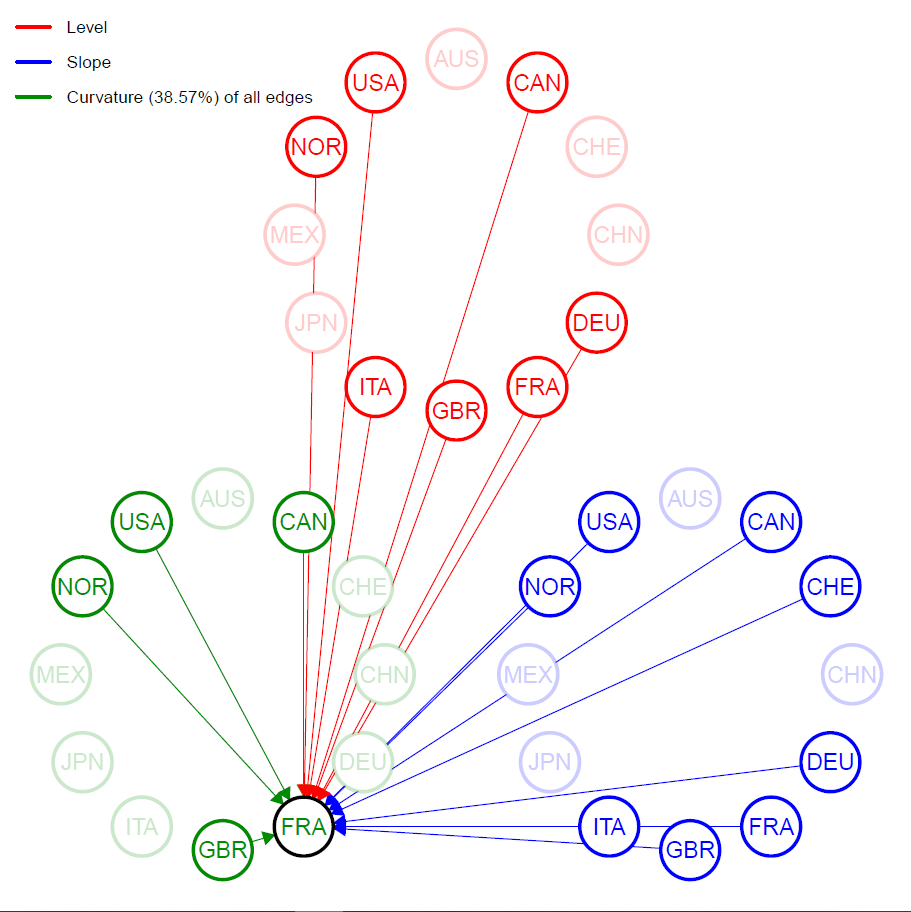
\includegraphics[width=13.5cm]{top_in}
\centering
\caption{Node having most incoming edges}

\end{figure}

%----------------------------------------------------------------------------------------------------------------------------------------------------

\subsection{Time series analysis}

%A statikus vizsgálódás után elvégzem az összekötöttségre vonatkozó dinamikus elemzést is. Gördülő időablakom hosszát 750 napnyinak választom meg. Ez 250 munkanapos évet feltételezve 3 évnek feleltethető meg. Minden egyes eltolással 5 napot ugrok, ami munkanapokat feltételezve egy hetet jelent. Így összesen 659 összekötöttséget reprezentáló modellt illesztek. Az ezekből kapott idősorokat mutatja az 5. ábra. A lila vonal a teljes hálózatra vonatkozó szignifikáns élek hányadát jelenti, a türkiz a különböző faktorok alhálózatainak összegét, míg a sárga a keresztkapcsolatok behúzott éleit jelképezi. A piros hátterű időszak a subprime válságra utal, míg a kék hátterű az európai adósságválságra. A periódusokat \cite{bostanci2020connected} alapján választom meg. Ezekben az időszakokban a hálózat összekötöttségi szintje megnövekszik.

After the static examination we performed a dynamic analysis of the factor interconnectedness. We chose a rolling window mrthod with size of 750 observations. Considering 250 business days long years, this can be interpreted as a three years long period. With each shifting we move 5 observations ahead which can be seen as one business week. By doing so, we define 659 separeted models. The time series coming from these models are shown on Figure \textcolor{magenta}{6}. Purple line stands for the ratio of the singnificant edges in the whole newtwork, cyan is the sum of the edges in different subnetworks and yellow represents edges coming from cross connections. As stated before, the subprime crysis is displayed by the red shaded area and the blue field covers the European sovereign debt.


%--------------------------------------------------------------------------Fig5--------------------------------------------------------------------------
\begin{figure}[H]
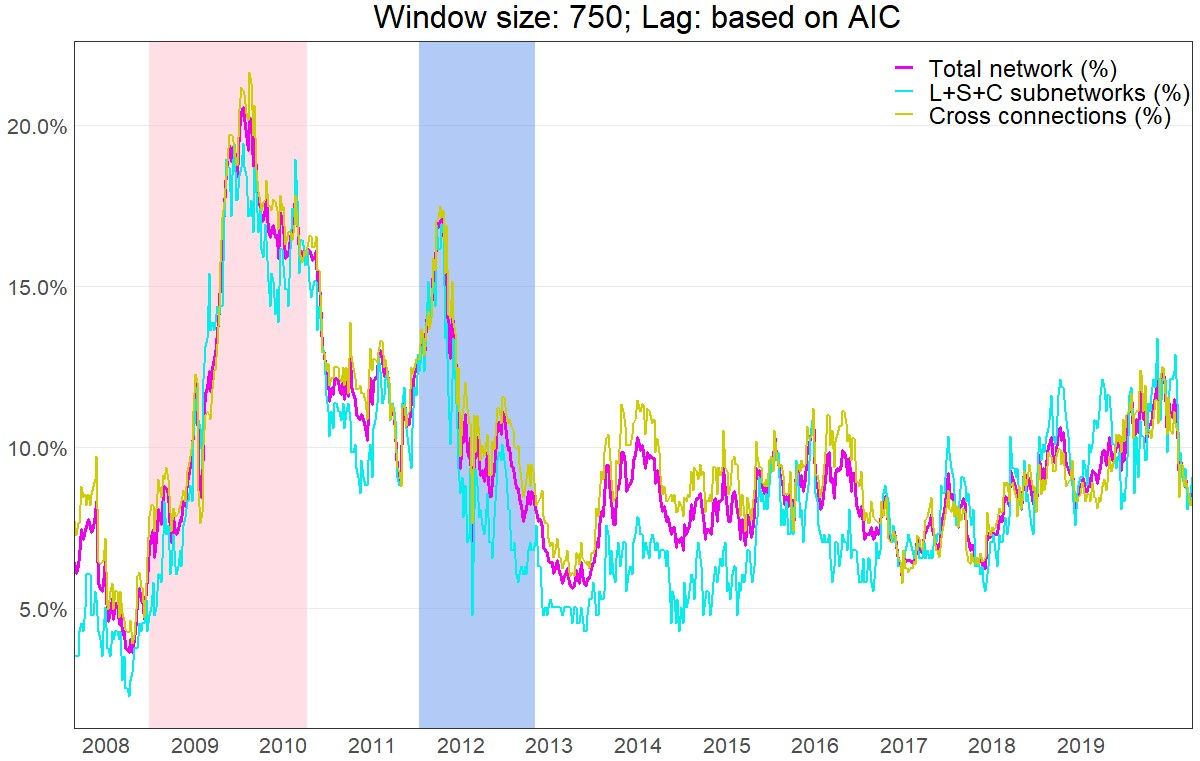
\includegraphics[width=11.5cm]{Time_series_750}
\centering
\caption{Dynamic Toda-Yamamoto analysis -  750 observations long window size}
\end{figure}

%A 6. ábra a vizsgált periódus alatt átlagosan letöbb nettósított éllel rendelkező faktorok idősorait mutatja. Ezek növekvő sorrendben: Norvégia Meredekség, USA Görbület és USA Szint. A subprime válság mindhárom faktorra hatással volt, itt az idősorok kiugró értékeket mutatnak. Norvégia Meredekség faktora az európai adósságválság ideje alatt emelkedett meg kimondottan. Ez azzal magyarázható, hogy 2011 végén Norvégia szuverén befektetési alapja eladta a teljes ír és portugál államadósság-állományát, és csökkentette spanyol és olasz kötvényinek tulajdonjogát.

Figure \textcolor{magenta}{7} shows the factors having the most edges during the whole observation period. In ascending order, these are Norwegian Slope, American Curvature and American Level. Subprime crisis had an effect on both three of them, time series have a peak during this period. The Slope factor of Norway increased drastically during the European Sovereign crisis. This can be explained by the fact that in the end of 2011, the sovereign investment fund of Norway sold whole of its Irish and Portugal sovereign debt, and decreased the ownership ratio in Spanish and Italian bonds.

%----------------------------------------------------------------------------------------------------------------------------------------------------

%--------------------------------------------------------------------------Fig6--------------------------------------------------------------------------
\begin{figure}[H]
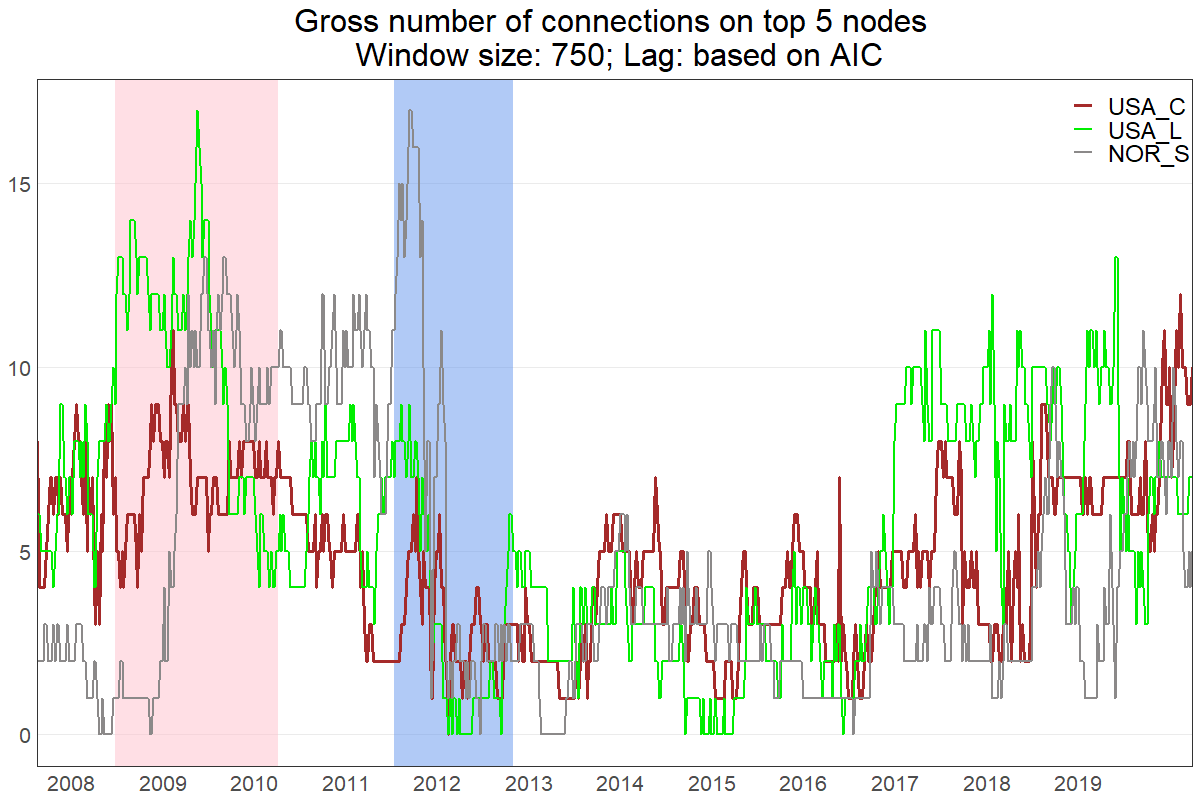
\includegraphics[width=11.5cm]{norway}
\centering
\caption{Edges having the most edges during the observation period - 750 observations long window size}
\end{figure}
%----------------------------------------------------------------------------------------------------------------------------------------------------

%A 6. táblázat az így kapott öt részidőszak átlagos éleinek számát mutatja be, faktoronkénti bontásban. Jól látható, hogy a subprime válság periódusa alatt minden élszám több, mint duplájára emelkedett. Ezután lassú csökkenés következett, a második válságos periódust a kapott számok nem is tükrözik. Ennek oka, hogy a 2008-as krízis a teljes világra kiterjedt, míg az európai adósságválság alapvetően az európai országokat (főképp az Euro-zónát) érintette. 

By defining two turbulent periods, which are colored on the plots, and three calm ones we devide our observation horizone to five subsets. Table \textcolor{magenta}{5} shows the average edge count for such periods aggregated by factors. One can see that during the subprime crisis, all of the edge numbers increases to more than double. This is followed by a slow decrease, the second turbulent period is not even represented by the numbers. The reason is that the crisis of 2008 was global, while the Europen soverein crisis had affect mainly on the European countries and especially on the Euro-zone.

%-----------------------------------------------------------------------------------table6------------------------------------------------------------------

\begin{table}[H]
\fontsize{10}{10}\selectfont
\centering% centering table
\begin{tabular}{l | cccccc}% creating eight columns
\hline\hline \\ [-1.5ex]                         %inserting double-line


		& 	Whole period  &	1. calm	&	1. crisis& 	2. calm& 	2. crisis&	 3. calm \\
\hline \\ [-1.5ex]  
Level	&		29	&	7	&	16.2	&	13.4	&  	12.1	&	 12\\
Slope	&		41	&	6	&	25.5	&	22.5	& 	16.2	& 	8.6\\
Curvature	&	23	&	7.3	&	20.7	&	9.7	& 	9.2	&	 9.9\\
Cross connections	&		225	&	61.8	&	142.2	&	109.1	& 	101.2	& 	76.1\\
%----------------------------------------------------------------------------------------------------------------------------------------------------

\hline            
\end{tabular}
\label{table:nonlin}% is used to refer this table in the text
\caption{Average edge count by edges during the five sub-periods - 750 observations long window size} %title of the table


\end{table}


\section{Robostness checks}

Yet to come...


\bibliographystyle{te}


\bibliography{research}

\begin{appendices}



\begin{table}[H]

\fontsize{10}{10}\selectfont
\centering % used for centering table
\begin{tabular}{l c c c c c c}% centered columns (4 columns)
\hline\hline   \\ [-1.5ex]               %inserts double horizontal lines
%Case & Method\#1 & Method\#2 & Method\#3 & test \\  [0.5ex]
Node & Average & St. dev & Minimum & Maximum & \textrho(1)  & \textrho(10) \\ [0.5ex] % inserts table %heading

\hline       \\ [-1.5ex]           % inserts single horizontal line
\textbf{\textit{Germany}} 	&		&		&		&		&		&	\\
1 year	&	0.026	&	1.628	&	-0.969	&	4.690	&	1.000	&	0.996	\\
5 years	&	0.026	&	1.632	&	-0.941	&	4.767	&	0.999	&	0.993	\\
10 years	&	0.024	&	1.545	&	-0.722	&	4.686	&	0.993	&	0.964	\\
												
30 years	&	0.023	&	1.448	&	-0.244	&	5.195	&	0.999	&	0.988	\\
\textbf{\textit{Italy}}	&		&		&		&		&		&		\\
1 year	&	0.024	&	1.533	&	-0.484	&	8.394	&	0.998	&	0.986	\\
5 years	&	0.024	&	1.520	&	0.237	&	7.895	&	0.998	&	0.985	\\
10 years	&	0.022	&	1.388	&	0.875	&	7.492	&	0.998	&	0.986	\\
												
30 year	&	0.019	&	1.197	&	2.043	&	7.584	&	0.998	&	0.985	\\
\textbf{\textit{France}}	&		&		&		&		&		&		\\
1 year	&	0.025	&	1.589	&	-0.801	&	4.657	&	1.000	&	0.996	\\
5 years	&	0.025	&	1.573	&	-0.773	&	4.910	&	0.999	&	0.993	\\
10 years	&	0.023	&	1.467	&	-0.415	&	4.851	&	0.999	&	0.991	\\
												
30 years	&	0.019	&	1.235	&	0.419	&	5.116	&	0.999	&	0.986	\\
\textbf{\textit{USA}}	&		&		&		&		&		&		\\
1 year	&	0.025	&	1.613	&	0.054	&	5.323	&	1.000	&	0.998	\\
5 years	&	0.019	&	1.232	&	0.559	&	5.301	&	0.999	&	0.980	\\
10 years	&	0.016	&	1.039	&	1.389	&	5.388	&	0.998	&	0.983	\\

30 years	&	0.015	&	0.962	&	1.992	&	5.839	&	0.997	&	0.976	\\
\textbf{\textit{Canada}}	&		&		&		&		&		&		\\
1 year	&	0.019	&	1.230	&	0.300	&	4.809	&	1.000	&	0.995	\\
5 years	&	0.018	&	1.146	&	0.484	&	4.801	&	0.999	&	0.989	\\
10 years	&	0.017	&	1.098	&	0.983	&	5.076	&	0.999	&	0.987	\\
												
30 years	&	0.016	&	1.012	&	1.306	&	5.612	&	0.998	&	0.985	\\
\textbf{\textit{Mexico}}	&		&		&		&		&		&		\\
1 year	&	0.032	&	2.025	&	1.512	&	10.570	&	0.979	&	0.988	\\
5 years	&	0.024	&	1.511	&	3.786	&	10.897	&	0.986	&	0.981	\\
10 years	&	0.021	&	1.352	&	4.619	&	12.413	&	0.992	&	0.970	\\

30 years	&	0.020	&	1.238	&	5.873	&	12.726	&	0.993	&	0.947	\\
\textbf{\textit{Japan}}	&		&		&		&		&		&		\\
1 year	&	0.004	&	0.272	&	-0.371	&	0.850	&	0.999	&	0.992	\\
5 years	&	0.008	&	0.485	&	-0.396	&	1.631	&	0.999	&	0.990	\\
10 years	&	0.010	&	0.656	&	-0.285	&	2.050	&	0.999	&	0.990	\\
												
30 years	&	0.012	&	0.761	&	0.053 	&	3.295	&	0.998	&	0.985	\\
\textbf{\textit{China}}	&		&		&		&		&		&		\\
1 year	&	0.012	&	0.730	&	0.957	&	4.382	&	0.992	&	0.966	\\
5 years	&	0.009	&	0.594	&	1.782	&	4.874	&	0.997	&	0.973	\\
10 years	&	0.009	&	0.570	&	2.481	&	5.503	&	0.993	&	0.964	\\
												
30 years	&	0.010	&	0.615	&	2.470	&	6.009	&		&		\\
\textbf{\textit{Australia}}	&		&		&		&		&		&		\\
1 year	&	0.028	&	1.775	&	0.675	&	7.376	&	0.999	&	0.992	\\
5 years	&	0.026	&	1.677	&	0.639	&	6.960	&	0.999	&	0.990	\\
10 years	&	0.024	&	1.497	&	0.885	&	6.873	&	0.999	&	0.988	\\
												
30 years	&	0.019	&	1.207	&	1.558	&	6.888	&	0.998	&	0.983	\\
\textbf{\textit{Norway}}	&		&		&		&		&		&		\\
1 year	&	0.022	&	1.410	&	0.199	&	6.243	&	0.999	&	0.994	\\
5 years	&	0.020	&	1.273	&	0.545	&	5.335	&	0.999	&	0.991	\\
10 years	&	0.019	&	1.194	&	0.888	&	5.276	&	0.999	&	0.989	\\
												
30 years	&	0.018	&	1.113	&	0.882	&	5.273	&	0.999	&	0.987	\\
\textbf{\textit{United Kingdom}}	&		&		&		&		&		&		\\
1 year	&	0.031	&	1.956	&	0.024	&	5.883	&	0.999	&	0.995	\\
5 years	&	0.026	&	1.644	&	0.161	&	5.821	&	0.999	&	0.991	\\
10 years	&	0.022	&	1.418	&	0.400	&	5.543	&	0.999	&	0.989	\\
												
30 years	&	0.018	&	1.110	&	0.939	&	5.070	&	0.999	&	0.987	\\
\textbf{\textit{Switzerland}}	&		&		&		&		&		&		\\
1 year	&	0.020	&	1.241	&	-1.165	&	3.375	&	1.000	&	0.996	\\
5 years	&	0.019	&	1.192	&	-1.196	&	3.200	&	0.999	&	0.993	\\
10 years	&	0.019	&	1.198	&	-1.138	&	3.455	&	0.999	&	0.991	\\
30 years	&	0.017	&	1.101	&	-0.644	&	3.733	&	0.998	&	0.986	\\

\hline%inserts single line
\end{tabular}
\label{table:nonlin}% is used to refer this table in the text
\caption{Descriptive statistics of country yield curve nodes}% title of Table
\end{table}
%----------------------------------------------------------------------------------------------------------------------------------------------------

\begin{table}

\fontsize{10}{10}\selectfont
\centering% centering table
\captionsetup{justification=centering}

%------------------------------------------------ ADF table----------------------------------------------------------------------------
\begin{subtable}[t]{1\textwidth}
\centering% centering table
\begin{tabular}{l cc cc cc cc cc cc}
\hline\hline \\ [-1.5ex]                         
 

Country	&	\multicolumn{2}{c}{DEU}			&	\multicolumn{2}{c}{ITA}			&	\multicolumn{2}{c}{FRA}			&	\multicolumn{2}{c}{USA}			&	\multicolumn{2}{c}{CAN}			&	\multicolumn{2}{c}{MEX}			\\[0.5ex] 

& value &P 		& value &P 			& value &P  		& value& P         			& value &P				& value &P\\

\hline       \\ [-1.5ex] 

Level	&	-2.30	&	0.45	&	-1.47	&	0.81	&	-2.16	&	0.51	&	-3.66	&	0.03	&	-3.06	&	0.13	&	-3.97	&	0.01	\\
Slope	&	-2.09	&	0.54	&	-2.26	&	0.47	&	-1.64	&	0.73	&	-1.50	&	0.79	&	-1.57	&	0.76	&	-1.88	&	0.63	\\
\medskip
Curvature	&	-2.22	&	0.49	&-3.59	&0.03	&	-2.36	&	0.43	&	-1.62	&	0.74	&	-2.35	&	0.43	&	-2.71	&	0.28	\\

\hline   \\ [-1.5ex]    

Country	&	\multicolumn{2}{c}{JPN}			&	\multicolumn{2}{c}{CHN}			&	\multicolumn{2}{c}{AUS}			&	\multicolumn{2}{c}{NOR}			&	\multicolumn{2}{c}{GBR}			&	\multicolumn{2}{c}{CHE}			\\

 & value &P & value &P& value &P & value &P& value &P & value &P\\

\hline       \\ [-1.5ex] 

Level	&	-2.97	&	0.17	&	-3.69	&	0.02	&	-2.90	&	0.20	&	-2.63	&	0.31	&	-2.16	&	0.51	&	-2.50	&	0.37	\\
Slope	&	-4.85	&	0.01	&	-3.69	&	0.03	&	-2.30	&	0.45	&	-2.72	&	0.27	&	-0.95	&	0.95	&	-3.14	&	0.10	\\
Curvature	&	-2.03	&0.57	&	-5.52	&	0.01	&	-2.61	&	0.32	&	-3.67	&	0.02	&	-1.62	&	0.74	&	-3.14	&	0.10	\\
\hline
\end{tabular}
\caption{\textbf{ADF test results}}
\end{subtable}
\hspace{\fill}
%----------------------------------------------------------------------------------------------------------------------------------------------------
\bigskip 

%------------------------------------------------ KPSS table----------------------------------------------------------------------------
\begin{subtable}[t]{1\textwidth}
\centering% centering table
\begin{tabular}{l cc cc cc cc cc cc}% creating eight columns
\hline\hline \\ [-1.5ex]                         %inserting double-line
%Audio Name&\multicolumn{2}{c}{Sum of Extracted Bits}&\multicolumn{4}{c}{Sum of Extracted Bits} \\ [0.5ex] 

Country	&	\multicolumn{2}{c}{DEU}			&	\multicolumn{2}{c}{ITA}			&	\multicolumn{2}{c}{FRA}			&	\multicolumn{2}{c}{USA}			&	\multicolumn{2}{c}{CAN}			&	\multicolumn{2}{c}{MEX}			\\[0.5ex] 

 & value &P & value &P& value &P & value &P& value &P & value &P\\

\hline       \\ [-1.5ex] 

Level	&	32.89	&	0.01	&	14.58	&	0.01	&	29.87	&	0.00	&	26.85	&	0.01	&	32.18	&	0.01	&	15.24	&	0.01	\\
Slope	&	4.26	&	0.01	&	7.61	&	0.01	&	4.50	&	0.01	&	5.30	&	0.01	&	5.40	&	0.01	&	4.78	&	0.01	\\
\medskip
Curvature	&	8.96	&	0.01	&	10.21	&	0.01	&	15.21	&	0.01	&	7.34	&	0.01	&	4.59	&	0.01	&	4.92	&	0.01	\\


\hline   \\ [-1.5ex]    

Country	&	\multicolumn{2}{c}{JPN}			&	\multicolumn{2}{c}{CHN}			&	\multicolumn{2}{c}{AUS}			&	\multicolumn{2}{c}{NOR}			&	\multicolumn{2}{c}{GBR}			&	\multicolumn{2}{c}{CHE}			\\

 & value &P & value &P& value &P & value &P& value &P & value &P\\

\hline       \\ [-1.5ex] 

Level	&	33.94	&	0.01	&	3.55	&	0.01	&	29.17	&	0.01	&	30.06	&	0.01	&	28.70	&	0.01	&	31.96	&	0.01	\\
Slope	&	33.21	&	0.01	&	14.99	&	0.01	&	7.32	&	0.01	&	1.25	&	0.01	&	7.53	&	0.01	&	5.49	&	0.01	\\
\medskip
Curvature	&	15.95	&	0.01	&	2.91	&	0.01	&	24.67	&	0.01	&	11.56	&	0.01	&	13.33	&	0.01	&	5.67	&	0.01	\\


\hline
\end{tabular}
\caption{\textbf{KPSS test results}}

\end{subtable}
\hspace{\fill}
%----------------------------------------------------------------------------------------------------------------------------------------------------
\bigskip

%------------------------------------------------ ADF(1) table----------------------------------------------------------------------------
\begin{subtable}[t]{1\textwidth}
\centering
\begin{tabular}{l cc cc cc cc cc cc}% creating eight columns
\hline\hline \\ [-1.5ex]                         %inserting double-line
%Audio Name&\multicolumn{2}{c}{Sum of Extracted Bits}&\multicolumn{4}{c}{Sum of Extracted Bits} \\ [0.5ex] 

Country	&	\multicolumn{2}{c}{DEU}			&	\multicolumn{2}{c}{ITA}			&	\multicolumn{2}{c}{FRA}			&	\multicolumn{2}{c}{USA}			&	\multicolumn{2}{c}{CAN}			&	\multicolumn{2}{c}{MEX}			\\[0.5ex] 

 & value &P & value &P& value &P & value &P& value &P & value &P\\

\hline       \\ [-1.5ex] 

Level	&	-17.05	&	0.01	&	-16.01	&	0.01	&	-15.99	&	0.01	&	-15.79	&	0.01	&	-16.35	&	0.01	&	-16.56	&	0.01	\\
Slope	&	-15.90	&	0.01	&	-14.62	&	0.01	&	-14.59	&	0.01	&	-16.55	&	0.01	&	-16.32	&	0.01	&	-15.19	&	0.01	\\
\medskip
Curvature	&-18.52	&	0.01	&	-18.67	&	0.01	&	-17.65	&	0.01	&	-17.45	&	0.01	&	-16.02	&	0.01	&	-18.88	&	0.01	\\


\hline   \\ [-1.5ex]    

Country	&	\multicolumn{2}{c}{JPN}			&	\multicolumn{2}{c}{CHN}			&	\multicolumn{2}{c}{AUS}			&	\multicolumn{2}{c}{NOR}			&	\multicolumn{2}{c}{GBR}			&	\multicolumn{2}{c}{CHE}			\\

 & value &P & value &P& value &P & value &P& value &P & value &P\\

\hline       \\ [-1.5ex] 

Level	&	-16.55	&	0.01	&	-16.99	&	0.01	&	-15.61	&	0.01	&	-16.43	&	0.01	&	-16.48	&	0.01	&	-15.57	&	0.01	\\
Slope	&		&		&	-18.90	&	0.01	&	-17.87	&	0.01	&	-17.61	&	0.01	&	-16.12	&	0.01	&	-14.59	&	0.01	\\
\medskip
Curvature	&	-17.51	&	0.01	&		&		&	-18.06	&	0.01	&	-17.04	&	0.01	&	-16.45	&	0.01	&	-14.27	&	0.01	\\



\hline
\end{tabular}
\caption{\textbf{ADF(1) test results}}
\end{subtable}
\hspace{\fill}
%----------------------------------------------------------------------------------------------------------------------------------------------------
\bigskip 

%------------------------------------------------ KPS (1) table----------------------------------------------------------------------------
\begin{subtable}[t]{1\textwidth}
\centering
\begin{tabular}{l cc cc cc cc cc cc}% creating eight columns
\hline\hline \\ [-1.5ex]                         %inserting double-line
%Audio Name&\multicolumn{2}{c}{Sum of Extracted Bits}&\multicolumn{4}{c}{Sum of Extracted Bits} \\ [0.5ex] 

Slope	&	\multicolumn{2}{c}{DEU}			&	\multicolumn{2}{c}{ITA}			&	\multicolumn{2}{c}{FRA}			&	\multicolumn{2}{c}{USA}			&	\multicolumn{2}{c}{CAN}			&	\multicolumn{2}{c}{MEX}			\\[0.5ex] 

 & value &P & value &P& value &P & value &P& value &P & value &P\\

\hline       \\ [-1.5ex] 

Level	&	0.04	&	0.10	&	0.13	&	0.10	&	0.06	&	0.10	&	0.03	&	0.10	&	0.06	&	0.10	&	0.08	&	0.10	\\
Slope	&	0.08	&	0.10	&	0.07	&	0.10	&	0.12	&	0.10	&	0.16	&	0.10	&	0.17	&	0.10	&	0.09	&	0.10	\\
Curvature	&	0.05	&	0.10	&	0.02	&	0.10	&0.05	&	0.10	&	0.08	&	0.10	&	0.08	&	0.10	&	0.01	&	0.10	\\


\hline   \\ [-1.5ex]    

Slope	&	\multicolumn{2}{c}{JPN}			&	\multicolumn{2}{c}{CHN}			&	\multicolumn{2}{c}{AUS}			&	\multicolumn{2}{c}{NOR}			&	\multicolumn{2}{c}{GBR}			&	\multicolumn{2}{c}{CHE}			\\

 & value &P & value &P& value &P & value &P& value &P & value &P\\

\hline       \\ [-1.5ex] 

Level	&	0.03	&	0.10	&	0.16	&	0.10	&	0.05	&	0.10	&	0.04	&	0.10	&	0.07	&	0.10	&	0.04	&	0.10	\\
Slope	&	0.03	&	0.10	&	0.03	&	0.10	&	0.04	&	0.10	&	0.08	&	0.10	&	0.24	&	0.10	&	0.14	&	0.10	\\
Curvature	&	0.06	&	0.10	&	0.05	&	0.10	&	0.04	&	0.10	&	0.03	&	0.10	&	0.16	&	0.10	&	0.05	&	0.10	\\


\hline
\end{tabular}
\caption{\textbf{KPSS(1) test results}}
\end{subtable}
\hspace{\fill}
%----------------------------------------------------------------------------------------------------------------------------------------------------
%\label{tab:table1}
\caption{Results of unit-root tests}
\end{table}

%----------------------------------------------------------------------------------------------------------------------------------------------------

%----------------------------------------------------------------------------------------------------------------------------------------------------

%----------------------------------------------------------------------------------------------------------------------------------------------------

\end{appendices}


\end{document}

